\documentclass[10pt]{iopart}
\usepackage[caption=false,font=normalsize,labelfont=sf,textfont=sf]{subfig}
\usepackage{enumitem}
\usepackage{outlines}
\usepackage{stfloats}
\usepackage{graphicx}

\newcommand{\gguide}{{\it Preparing graphics for IOP Publishing journals}}
\usepackage[numbers,sort&compress]{natbib}

\DeclareRobustCommand*{\numrefmark}[1]{%
  \raisebox{-1.5pt}[0pt][0pt]{\textsuperscript{\scriptsize\ensuremath{#1}}}}

\newcommand{\customfootnote}[2]{\begingroup\renewcommand\thefootnote{#1}%
\footnotetext{#2}}

\begin{document}

\title[DR-SENS for Haptic Feedback]{Distally-Referred Surface Electrical Nerve Stimulation (DR-SENS) for Haptic Feedback}

\author{Luis Mesias\numrefmark{1}\textsuperscript{,}\numrefmark{2}\textsuperscript{,}\numrefmark{4}, 
M. Akif Gormez\numrefmark{2}\textsuperscript{,}\numrefmark{4}, 
Dustin Tyler\numrefmark{1}\textsuperscript{,}\numrefmark{3}\textsuperscript{,}\numrefmark{5}\textsuperscript{,}\numrefmark{6},  
Nathan Makowski\numrefmark{4}, 
Emily L. Graczyk\numrefmark{1}\textsuperscript{,}\numrefmark{3}\textsuperscript{,}\numrefmark{7} 
and Michael J. Fu\numrefmark{1}\textsuperscript{,}\numrefmark{2}\textsuperscript{,}\numrefmark{4}\textsuperscript{,}\numrefmark{7}}

\address{Case Western Reserve University, 10900 Euclid Ave., Cleveland, Ohio, US}
\ead{lem136@case.edu and mjf24@case.edu}
\vspace{10pt}
\begin{indented}
\item[]June 2023
\end{indented}


\customfootnote{}{%
{\scriptsize
\textsuperscript{\numrefmark{1}}Human Fusions Institute, Case Western Reserve University (CWRU); %
\textsuperscript{\numrefmark{2}}Dept. of Electrical, Computer, and Systems Engineering, CWRU;% 
\textsuperscript{\numrefmark{3}}Dept. of Biomedical Engineering, CWRU; %
\textsuperscript{\numrefmark{4}}Dept. of Physical Medicine \& Rehabilitation, The MetroHealth System; %
\textsuperscript{\numrefmark{5}}Advanced Platform Technology Center, Dept. of VA Northeast Ohio Healthcare System; %
\textsuperscript{\numrefmark{6}}Afference Inc.; %
\textsuperscript{\numrefmark{7}}These authors contributed equally %
}}

\begin{abstract}

\textbf{Objective:}
This study introduces distally-referred surface electrical nerve stimulation (DR-SENS) and evaluates the effects of electrode placement, polarity, and stimulation intensity on the location of elicited sensations in able-bodied individuals.
\textbf{Approach:} 
%Due to the large search space of electrode combinations and stimulation parameters, 
A two-phased human experiment was used to characterize DR-SENS. In Experiment One, we explored 182 electrode combinations to identify a subset of electrode position combinations that would be most likely to elicit distally-referred sensations isolated to the index finger without discomfort. In Experiment Two, we further examined this subset of electrode combinations to determine the effect of stimulation intensity and electrode position on perceived sensation location. Stimulation thresholds were evaluated using parameter estimation by sequential testing and sensation locations were characterized using psychometric intensity tests.
\textbf{Main Results:}
We found that electrode positions distal to the wrist can consistently evoke distally referred sensations with no significant polarity dependency. The finger-palm combination had the most occurrences of distal sensations, and the different variations of this combination did not have a significant effect on sensation location. Increasing stimulation intensity significantly expanded the area of the sensation, moved the most distal sensation distally, and moved the vertical centroid proximally. Also, a large return electrode at the elbow mitigated all sensation at the return electrode site while using symmetric stimulation waveforms. Furthermore, this study showed that the most intense sensation for a given percept can be distally referred. Lastly, for each subject, at least one of the finger-palm combinations evaluated in this study worked at both perception threshold and maximum comfortable stimulation intensities. 
\textbf{Significance:}
These findings show that a non-invasive surface electrical stimulation charge modulated haptic interface can be used to elicit distally-referred sensations on able-bodied users. Furthermore, these results inform the design of novel haptic interfaces and other applications of surface electrical stimulation based haptic feedback on electrodes positioned distally from the wrist. 

\end{abstract}

\vspace{2pc}
{\footnotesize \noindent{\it Keywords}: Distally-Referred Sensation, Haptic Feedback, Surface Electrical Stimulation}
\maketitle
\ioptwocol

\section{Introduction}
Tactile information at the fingertips is important for detection of object contact and grasp force modulation, as the fingertips come into contact with objects in most grasp configurations \cite{johansson_coding_2009}. Many tactile haptic feedback modalities (displays) have been developed to enhance the immersiveness of virtual reality (VR) and mixed reality (MR) environments \cite{wang_haptic_2019}. Typically, tactile displays are designed to mimic veridical interactions between the hand and the environment by applying mechanical or electrical stimulation where the user's hand or skin makes contact with the haptic device. These devices include robotic haptic handles, exoskeleton gloves, vibrotactile motors, tactile arrays of micro-actuators (ultrasonic, pneumatic, or mechanical), or electrotactile stimulation electrodes.\cite{ma_rml_2015, manus_prime_nodate, haptx_haptic_nodate, akifieva_teslasuit_2019, hayden_these_2022}. However, these existing approaches typically interact directly with the pads of the fingers and occlude the fingertip completely, which is not ideal for MR applications in which the user must also grasp and use veridical objects while interacting with virtual objects. Thus, there is a need for a tactile display that provides sensations to the fingertip without occluding the fingertip. As part of a semifinal entry to the Avatar XPRIZE competition \cite{zhangoperator}, we developed an innovative tactile display, which we termed distally-referred surface electrical nerve stimulation (DR-SENS), that evokes tactile sensations at the fingertips using surface electrodes positioned up to 1-2 centimeters away from each fingertip. The present study presents an investigation into the ability of our novel DR-SENS approach to evoke comfortable and useful tactile sensations on the finger that are perceived at a location that is distal to the electrode position. 

In DR-SENS, the goal is to primarily activate the digital nerves on the hand that innervate the fingertip, while avoiding activation of the fingertip's cutaneous sensory receptors. This approach activates axons of passage, which has the potential to generate more natural-feeling sensations located distal to the electrode location \cite{dalonzo_hyve_2014,geng_evaluation_2012}. This differs from fingertip electrotactile displays, which target sensory receptors to elicit unnatural paresthesia sensations directly under the electrode and use frequency modulation to communicate haptic information \cite{kajimoto_tactile_1999, kitamura_electrotactile_2015}. \citeauthor{kajimoto_tactile_1999} first observed distally-referred paresthesia when altering the polarity of fingertip electrotactile arrays and described the phenomenon as an undesirable ``sensory-shift'' from the location of the electrode, since the goal was to precisely elicit paresthesia over a particular electrode \cite{kajimoto_tactile_1999}. They proposed that cathodic current sources elicit sensations under the electrode by targeting the Meissner corpuscle and anodic current sources elicit sensory-shift sensations distal to the electrode by targeting and Pacinian corpuscle and Merkel cell mechanoreceptors that run distally along the finger. Polarity-induced sensory-shift was then purposely used to elicit sensations on the fingertip without having an electrode between the fingertip and a stylus tool \cite{yoshimoto_development_2011}. Most recently, \citeauthor{tanaka_full-hand_2023} demonstrated that electrodes positioned on the posterior side of the finger can elicit paresthesia sensations on the palmar side of the hand without eliciting sensations on the dorsal side if stimulation current is maintained just above the perception threshold intensity of the anterior side. It was presumed that this is possible because there are more sensory receptors on the palmar side of the hand than the dorsal side. However, a limitation of this approach is that the intensity of the perceived stimulation cannot be increased without causing sensations to be felt on both the posterior and anterior surfaces of the hand \cite{tanaka_full-hand_2023}.

Distally-referred stimulation was also used for sensory restoration purposes on individuals with limb loss to elicit a sensation on the amputated limb by placing electrodes on the residual limb. Sensory restoration literature suggests that unnatural sensations are mainly localized near the stimulating electrodes \citeauthor{pena_channel-hopping_2021}, and that distally-referred sensations were more commonly classified as ``natural'' \cite{slopsema_natural_2018, pena_channel-hopping_2021}. Specifically, electrodes placed on the forearm near the ulnar, radial, and median nerves simultaneously elicited paresthesia that was perceived on the skin surrounding the electrodes, along with more natural sensations (described by participants as tapping, knocking, touch, and pressure \cite{dalonzo_electro-cutaneous_2018, slopsema_natural_2018}) that were perceived distal to the electrodes\cite{dalonzo_hyve_2014,geng_evaluation_2012}. These results from studies on the forearm led to our overall hypothesis that distally-referred sensations isolated to an individual finger could be elicited by placing electrodes near the digital nerves of the hand. 

DR-SENS has the potential to become an innovative haptic display for people both with and without limb loss. However, prior sensory restoration studies have focused on electrode positions proximal to the wrist for people with limb loss, because the wrist and areas distally positioned from it have been lost due to amputation. Prior sensory restoration studies have not evaluated skin-surface electrode positions distally positioned from the wrist for  people without limb loss as the end users. Some of the electrode positions evaluated in these studies are the residual limb's upper arm \cite{vargas_evoked_2019, henry_shin_evoked_2018}, elbow \cite{forst_surface_2015, slopsema_natural_2018}, or forearm \cite{pena_channel-hopping_2021,danna_somatotopic_2017}. Previous sensorized prosthesis studies have shown that stimulating the tricjpg area can provide information about object stiffness, shape, and surface topology \cite{vargas_object_2020, vargas_evoked_2019}. Proximal electrode positions on the forearm or upper arm often lead to poor sensation location selectivity because the sensation locations cover vast areas of the hand. This mismatch between perceived sensation location and the location of the hand that is interacting with the environment can lead to increased cognitive load and response time during object manipulation tasks\cite{pena_channel-hopping_2021}. \citet{dalonzo_electro-cutaneous_2018} investigated electrode positions in the palms of people with partial hand amputations and reported that some participants felt sensations isolated to individual fingers. These results suggest that using more distal electrode positions on the hand might provide better sensation location selectivity because the afferents serving the fingers are spatially separated in the palm. Another benefit of distally positioned electrodes is that distal regions of hand nerves only contain sensory afferents, so electrical stimulation is less likely to activate muscles, unlike in more proximal regions of nerves in which spillover into motor fascicles can lead to undesired muscle activation. Distal electrode positions activate muscle fascicles less often than proximal electrode positions because all motor efferents have branched out from the nerve at more proximal locations.

Alternatively, electrotactile display studies have focused on electrode positions distally located from the wrist, with a focus on electrodes located on the fingers and the use of frequency modulation \cite{kajimoto_tactile_1999, yoshimoto_development_2011, yoshimoto_roughness_2014, kitamura_electrotactile_2015}. \citeauthor{scarpelli_evoking_2020} showed that the area of the sensation elicited changed proportionally to changes in stimulation intensity for both charge and frequency modulation, but charge modulation sensations were described as natural and frequency modulation sensations were described as tingling/vibration \cite{scarpelli_evoking_2020}. All prior frequency modulation approaches have a limitation that the intensity is coupled to the frequency of the perceived sensation. For example, at low intensity the perceived sensation resembles a low-frequency pulsing as the stimulation frequency is reduced, but as frequency is increased to increase sensation intensity, the sensation becomes fused and feels constant \cite{graczyk_frequency_2022}.

Haptic displays should convey the stimulus intensity, and an alternative to frequency modulation is charge modulation. It has been previously shown that increasing pulse amplitude or pulse width (charge modulation) in implanted nerve interfaces increases the perceived intensity of the sensation \cite{tan_neural_2014, graczyk_neural_2016}. Therefore, an increase in stimulation intensity might also be effective in conveying the intensity of a stimulus delivered via DR-SENS. Prior studies have examined the stimulation parameters that determine sensory detection threshold, which is the combination of pulse widths and current amplitudes that generate the minimally perceptible sensation \cite{slopsema_natural_2018,forst_surface_2015,pena_channel-hopping_2021, tanaka_full-hand_2023}. However, it is unknown how these threshold stimulation parameters will change for more distal electrode positions on the palm and fingers and how perceived sensation location changes as stimulation intensity increases from perception threshold up to the maximum comfortable limit. Another critical requirement for haptic displays is that the evoked sensations should be comfortable to the user throughout this intensity range. The current work will expand on previous work by evaluating how perceived sensation locations change for different electrode positions and charge modulation intensities.

Therefore, there is a need to systematically explore electrode positions distal to the wrist in people without limb loss that can generate distally-referred sensations with location selectivity while using charge modulation, which is the primary goal of the current study. 

Our long-term goal is to use DR-SENS as a novel haptic display modality for able-bodied users. As an initial step toward this goal, we hypothesized that electrode positions distal to the wrist can generate distally-referred sensations without discomfort or muscle activation and can elicit sensations isolated to an individual finger. The current work investigated this hypothesis by rigorously surveying electrode positions distal to the wrist and characterizing the associated locations of the perceived sensations. Due to the large search space of electrode combinations and stimulation parameters, a two-phased human experiment was used to characterize DR-SENS in able-bodied humans, which was developed to make the number and duration of study visits more practical for subjects. In Experiment One, we explored a broad range of electrode positions to identify a subset of useful electrode position combinations that would be most likely to elicit distally-referred sensations without discomfort that are isolated to a single finger. In Experiment Two, we further examined the useful electrode combinations identified in Experiment One to determine if changes in stimulation parameters resulted in changes to the perceived sensation location. In both sets of experiments, we focused on evoking sensation on the index finger due to its importance in both object grasp and haptic search tasks. 

\section{Experiment One: Identify electrode combinations that elicit distally-referred index finger sensations}\label{sec:phase1}

Experiment One focused on the effects of inter-electrode distance, electrode position and polarity on generating distally-referred sensations to the index finger.

\subsection{Experiment One: Methods}

\paragraph{Participants and Study Visits:} Five able-bodied participants (two female, three male; age 28 $\pm$ 6 years (mean $\pm$ standard deviation)) performed the experiment in a single 3.5-hour long session. All participants provided written informed consent to participate in these experiments, which were approved by the Metro Health System Institutional Review Board. 

\paragraph{Stimulation System and Parameters:}These experiments used an investigational grade stimulator custom-designed at Case Western Reserve University \cite{trier_modular_2001}. The stimulator can generate currents between 1 mA and 100 mA with a 1 mA resolution and pulse widths between 0 $\mu$s and 255 $\mu$s with a 1 $\mu$s resolution. The stimulator was controlled by a custom MATLAB Simulink model on a host computer for the selection of stimulation parameters. Disposable self-adhesive Ag$|$AgCl electrodes with a 1.8 cm diameter (Axelgaard Manufacturing CO., LTD, Lystrup, Denmark) were connected to the stimulator. The stimulator generated a cathode-first, charge balanced, current controlled, symmetric output square waveform. The stimulation was applied for five seconds at 90 Hz in order to generate continuous sensations \cite{graczyk_frequency_2022}. 

\paragraph{Identification of Possible Electrode Positions:} \label{sec:PossibleElectrodes} At the beginning of each session, the participant's hands were prepped with TENS wipes (Covidien, Mansfield, MA). Each participant's left hand and index finger were divided into 14 regions (Fig. \ref{fig:electrodes_positions}), consisting of 8 regions in the index finger (IA, PA, IP, PP, IL, PL, IM and PM) and 6 regions on the palm (PA1, PA2, PA3 and PP1, PP2, PP3). These 14 regions, referred to subsequently as `electrode positions', were placed close to the digital nerve branch of the median nerve that innervates the index finger. Each of the 8 regions on the finger were located at the center of either the intermediate or proximal phalanges on each of the faces of the finger (medial, lateral, posterior, and anterior). The distal phalange was not evaluated because it is the target location for the elicited sensation, and because it would not be possible to elicit sensation distal to it. A distally-referred sensation was defined as a sensation located distally from the most distal electrode position, so electrode positions on the distal phalange cannot elicit this type of sensation because they are on the most distal section of the finger. For the finger regions, the naming convention is a combination of the finger segment (intermediate or proximal phalange) and the face of the segment (anterior, posterior, medial, or lateral) described above. For example, the electrode positions on the proximal phalange's lateral face is the PL electrode position (see Fig. \ref{fig:electrodes_positions} caption). The six palm electrode positions were defined while the participant's hand was laid on a flat surface and a guide line was drawn through the center of the finger on the posterior side of the hand. The distance along this guide line from the knuckle to a horizontal line running through the Ulnar styloid process was measured, and a point was placed every third of the distance (Fig. \ref{fig:electrodes_positions}). The same process was repeated for the anterior side of the hand. In the naming convention for the palm electrode positions, the first letter is always P for palm, the second letter stands for the side of the palm (anterior or posterior), and the number is the distance from the finger in terms of thirds. 

To ensure the electrode positions were consistent throughout the study, each of these positions was marked on the participant’s hand using a skin-safe marker. This methodology ensured repeatability across participants regardless of hand size by using anatomical landmarks. Each electrode position can have both polarities (active and return), so a total of 182 (14 × 13) electrode position combinations were evaluated (referred to subsequently as electrode combinations).

\begin{figure}
  \centering
  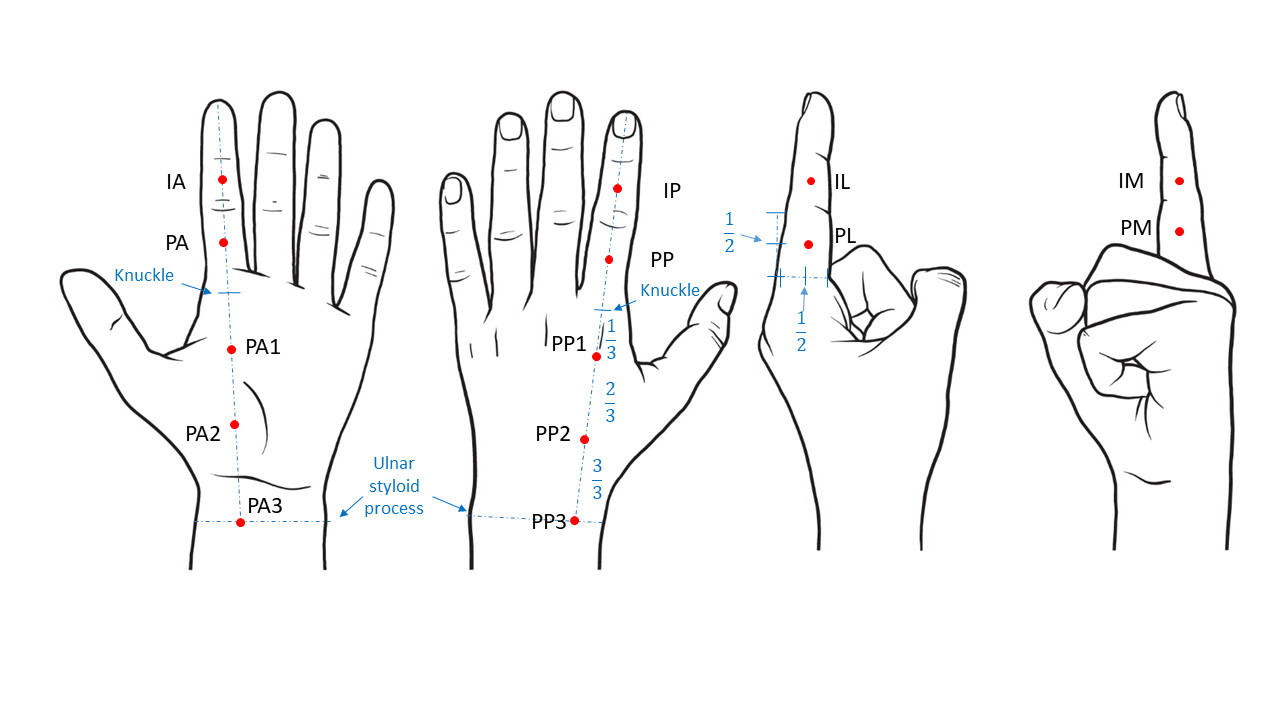
\includegraphics[width=0.5\textwidth,trim={1.5cm 5cm 1cm 2.2cm},clip]{fig/Image_Hand.jpg}
  \caption{The 14 electrode positions for Experiment 1 are indicated by red dots. Positions on the finger were centered on the surface of the following phalanges: intermediate anterior (IA) and posterior (IP), proximal anterior (PA) and posterior (PP), intermediate lateral (IL) and medial (IM), and proximal lateral (PL) and medial (PM). Palm posterior (PP) and anterior (PA) positions were distributed 1/3 (PP1, PA1) and 2/3 (PP2, PA2) and 3/3 (PP3, PA3) of the distance from the knuckle to the horizontal plane of the ulnar styloid process.}
  \label{fig:electrodes_positions}
\end{figure}


\paragraph{Assessing Electrode Combinations:}
Participants were first asked to find their maximum comfortable limit. To ensure that each participant's maximum comfortable limit was less than 255 $\mu$s (maximum pulse width of the stimulator), the pulse amplitude was set higher (15 mA) than the 3 mA amplitude that was reported in the literature to have elicited sensations \cite{pena_channel-hopping_2021, dalonzo_electro-cutaneous_2018}. Each participant was asked to control pulse width using the scroll wheel of a computer mouse, so they could limit exposure to pulse widths that produced uncomfortable sensations. Participants were then instructed to find the discomfort threshold by increasing pulse width until discomfort was felt, and then to immediately decrease pulse width to find the highest pulse width that produced comfortable sensation without discomfort. The simulation was turned on for five seconds at a time to avoid possible desensitization. To make sure the participant had enough time to adjust the pulse width and judge the sensation, additional 5-second stimulation trains were applied if necessary. To minimize variability related to electrode reapplication, each electrode combination was assessed for both polarities without moving the electrodes. Additionally, one of the electrode positions was kept constant while the other was repositioned to the 13 other electrode positions. This process was repeated a total of 14 times to cover all 182 different electrode combinations. The electrodes were replaced as necessary throughout the session to ensure adequate adhesion of the electrode to the skin. 

The participant was asked three questions for each stimulus: 1) Is the sensation distal to the electrode position (yes or no)?  2) Is the sensation comfortable (yes or no)? and 3) Do you feel any muscle contraction from the stimulation (yes or no)? Prior to beginning the experiment, the researcher clarified the instructions with the participant and the participant was able to ask questions to improve understanding. Only electrode combinations in which the participant answered 'yes' to both questions 1 and 2 and 'no' to question 3 were classified as ``useful'' sensations and were selected for further analysis.

\paragraph{Data Analysis:}
To compare different electrode positions and combinations, the data was averaged across all five participants. When comparing across different polarity conditions, data was average across subjects to assess different electrode combinations and average across electrode combinations to assess differences between subjects. The polarity data was assessed for normality using a quantile-quantile (Q-Q) plot and histograms, but the data did not fit a normal distribution. Therefore, a non-parametric test, Kruskal-Wallis rank sum test, was used to investigate if there was a significant difference among polarity conditions. A post hoc pairwise comparison was run using Dunn’s Test for Multiple Comparisons with a Bonferroni adjustment. 

\subsection{Experiment One: Results}
Data was pooled across subjects and trials to determine how electrode position impacted the frequency of reports of useful sensations. The top half electrode positions that were most often associated with a useful classification, in descending order (from most frequently useful to least frequently useful), were PA1, IL, IA, PL, IM, IP, and PA (Fig. \ref{fig:explo_elec}). The electrode positions that were least often associated with a useful classification were PA3, PP3, PP, PP2, PA2, PM, PP1 in ascending order (from least frequently useful to most frequently useful). Most of the least useful electrode positions were proximal palm electrode positions ($5/7$). When looking at the different types of electrode combinations, 68\% (n=480)of the trials with finger-palm electrode combinations (one electrode position in the palm and one in the finger) were classified as useful (Fig. \ref{fig:explo_comb}). In contrast, only 23\% (n=150) of the palm-palm electrode combination trials were classified as useful. The top three electrode positions on the palm were PA1, PP1, and PA2, and the top three finger electrode positions were IL, IA, and PL. Based on these results, finger-palm combination with a proximal palm electrode and a finger could elicit distally-referred sensation. The finger-palm combinations using the top three finger and palm electrodes were as follows IA-PA1 (100\% useful, n=10), IL-PA1 (100\% useful, n=10), PL-PA1 (90\% useful, n=10), IA-PP1 (90\% useful, n=10), IL-PP1 (100\% useful, n=10), PL-PP1 (90\% useful, n=10), IA-PA2 (90\% useful, n=10), IL-PA2 (100\% useful, n=10), PL-PA2 (70\% useful, n=10). Also, the positions of both the active and return electrode can affect the presence of distally-referred sensations. 

\begin{figure*}
    \centering
    \subfloat[]{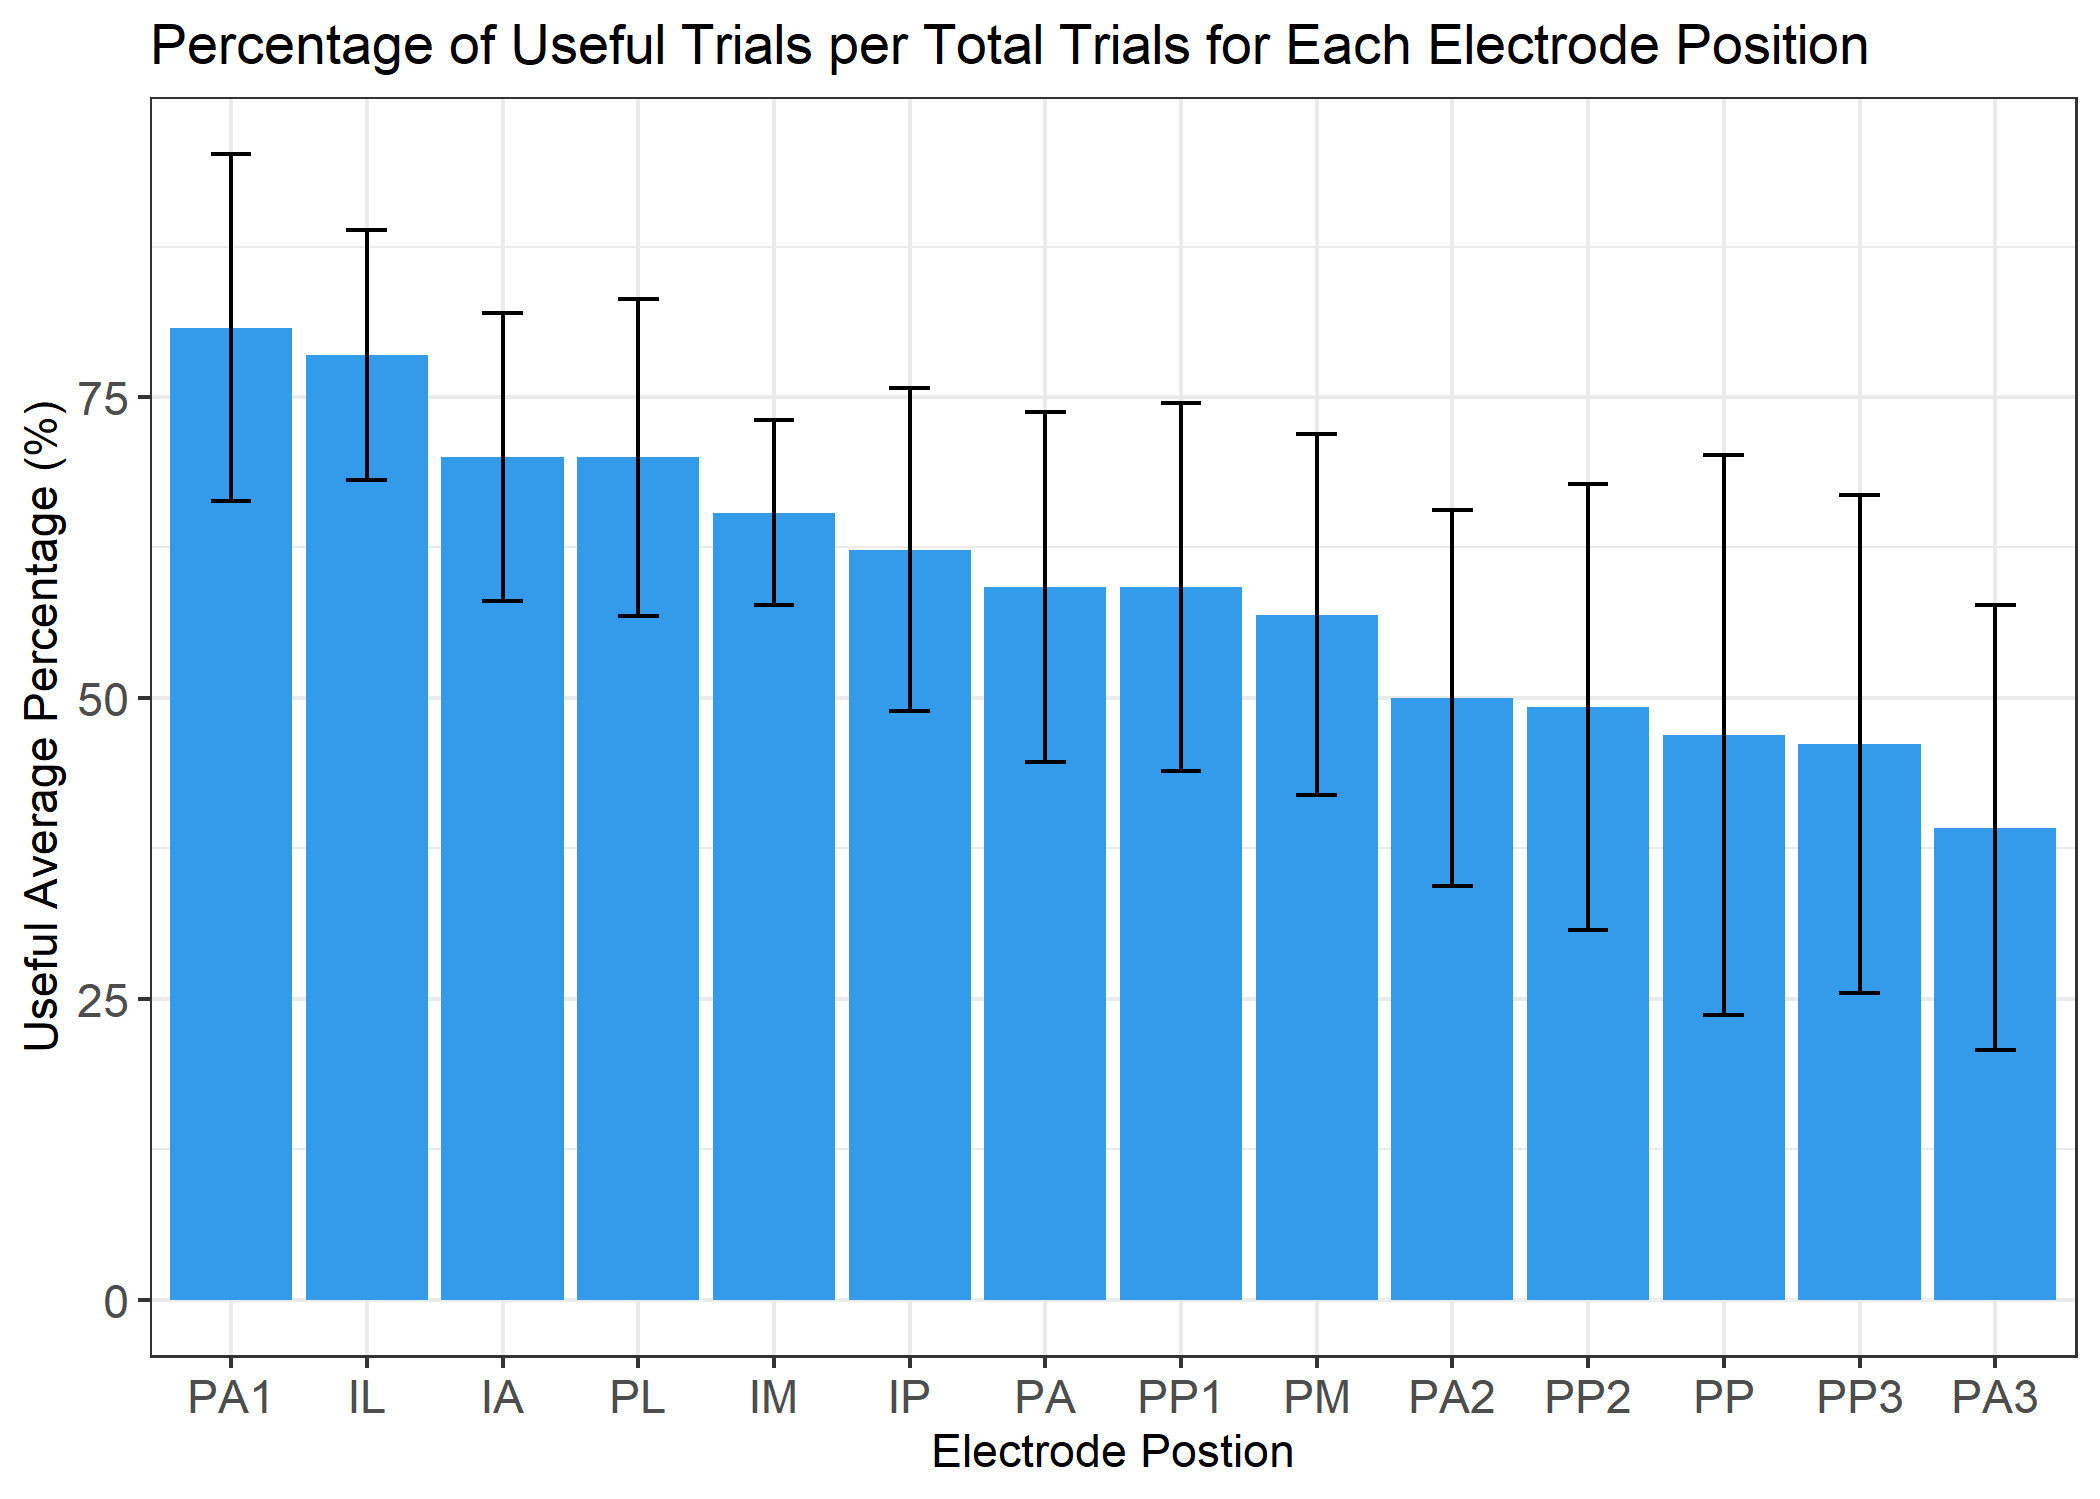
\includegraphics[width=0.48\textwidth,clip]{fig/explo_res_elec.jpg}
    \label{fig:explo_elec}}
    \subfloat[]{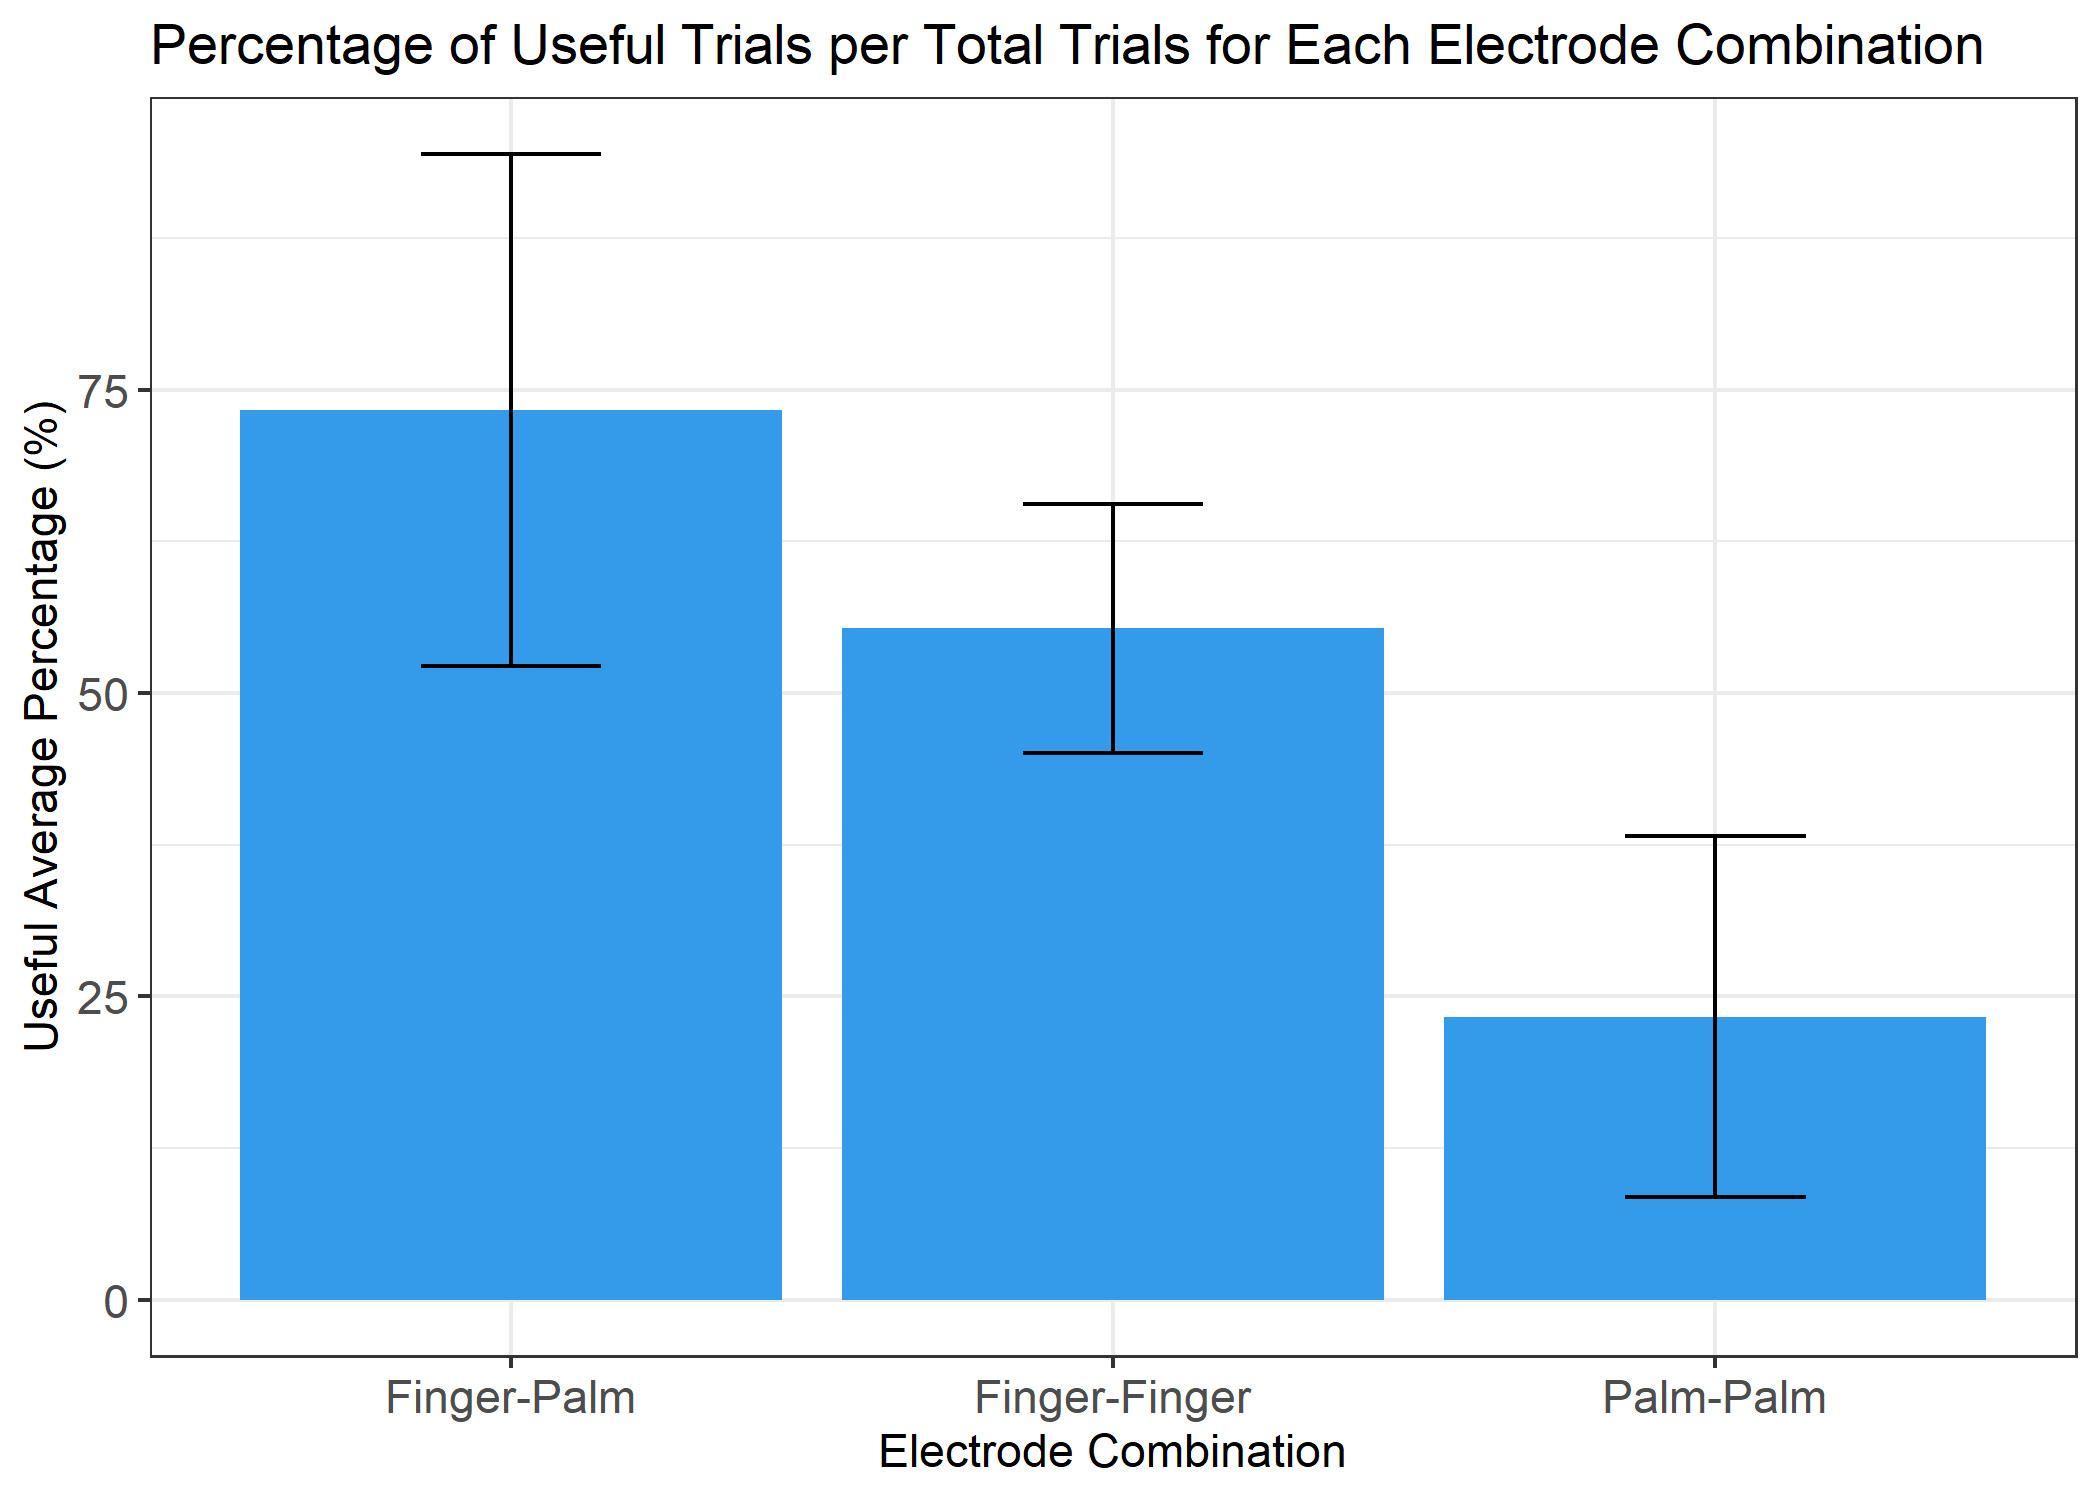
\includegraphics[width=0.48\textwidth,clip]{fig/explo_res_combination.jpg}
    \label{fig:explo_comb}}
    \caption{Average percentage and standard deviation of useful trials (\ref{fig:explo_elec}) for each electrode position relative to the total number of trials where the specific electrode was used across all subjects (n=130 per electrode position) and (\ref{fig:explo_comb}) for each electrode combination relative to all the trials where electrodes were positioned on the positions described by the combination (e.g. finger and palm) across all subjects (n=280 finger-finger, n=480 finger-palm, n=150 palm-palm).}
    \label{fig:explo_elec_comb}
\end{figure*}

For a given electrode combination, there are two possible arrangements  that depend on the relative positions of the active and return electrodes. For example, a given finger-palm electrode configuration can have the active electrode positioned on the palm with the return on the finger, or vice versa. The difference between these two arrangements is polarity. On average, participants reported 71\% (n=910) of the perceived sensations were polarity independent (PI) across all electrode combinations (Fig \ref{fig:explo_polarityComb}). There was a significant difference between different polarity conditions (Kruskal-Wallis rank sum test, $p<0.001$). The post hoc analysis reveled there was a statistically significant difference between PI trials and the polarity dependent conditions (Dunn (1964) Kruskal-Wallis multiple comparison: PI vs. Cathodic on distal, $p<0.001$; PI vs. Cathodic on proximal, $p=0.029$; PI vs. same phalange, $p<0.001$). For polarity dependent trials, there was no clear pattern across finger-finger and finger-palm electrode combinations. However, for palm-palm electrode combinations, a greater number of useful sensation trials were reported when the active electrode was the most distal electrode position (i.e. the cathodic-leading pulse was provided to the most distal electrode of the pair). There was no significant difference among the polarity dependent conditions (Dunn Kruskal-Wallis multiple comparison: Cathodic on distal vs. Cathodic on proximal, $p=0.90$; Cathodic on distal vs. same phalange, $p=1.00$; Cathodic on proximal vs. same phalange, $p=0.74$). When looking at similarities within subjects, must subjects showed little polarity dependence, except for subject three (Fig. \ref{fig:explo_polaritySub}). When looking at the polarity dependence within subjects, most of these polarity dependent useful trials occurred when the leading pulse on the most distal electrode position was cathodic.

\section{Experiment Two: Effect of Stimulation Parameters and Electrode Position on Distally-Referred Sensations}

In Experiment Two, a subset of electrode positions that most frequently elicited useful distally-referred sensations (based on the results of Experiment One) were examined more rigorously and in a larger number of participants. The goal of Experiment Two was to characterize how the location of distally-referred sensations at the index finger can change when the stimulation intensity varied between the perception threshold and the maximum comfortable limit.

\begin{figure*} [t]
    \centering
    \subfloat[]{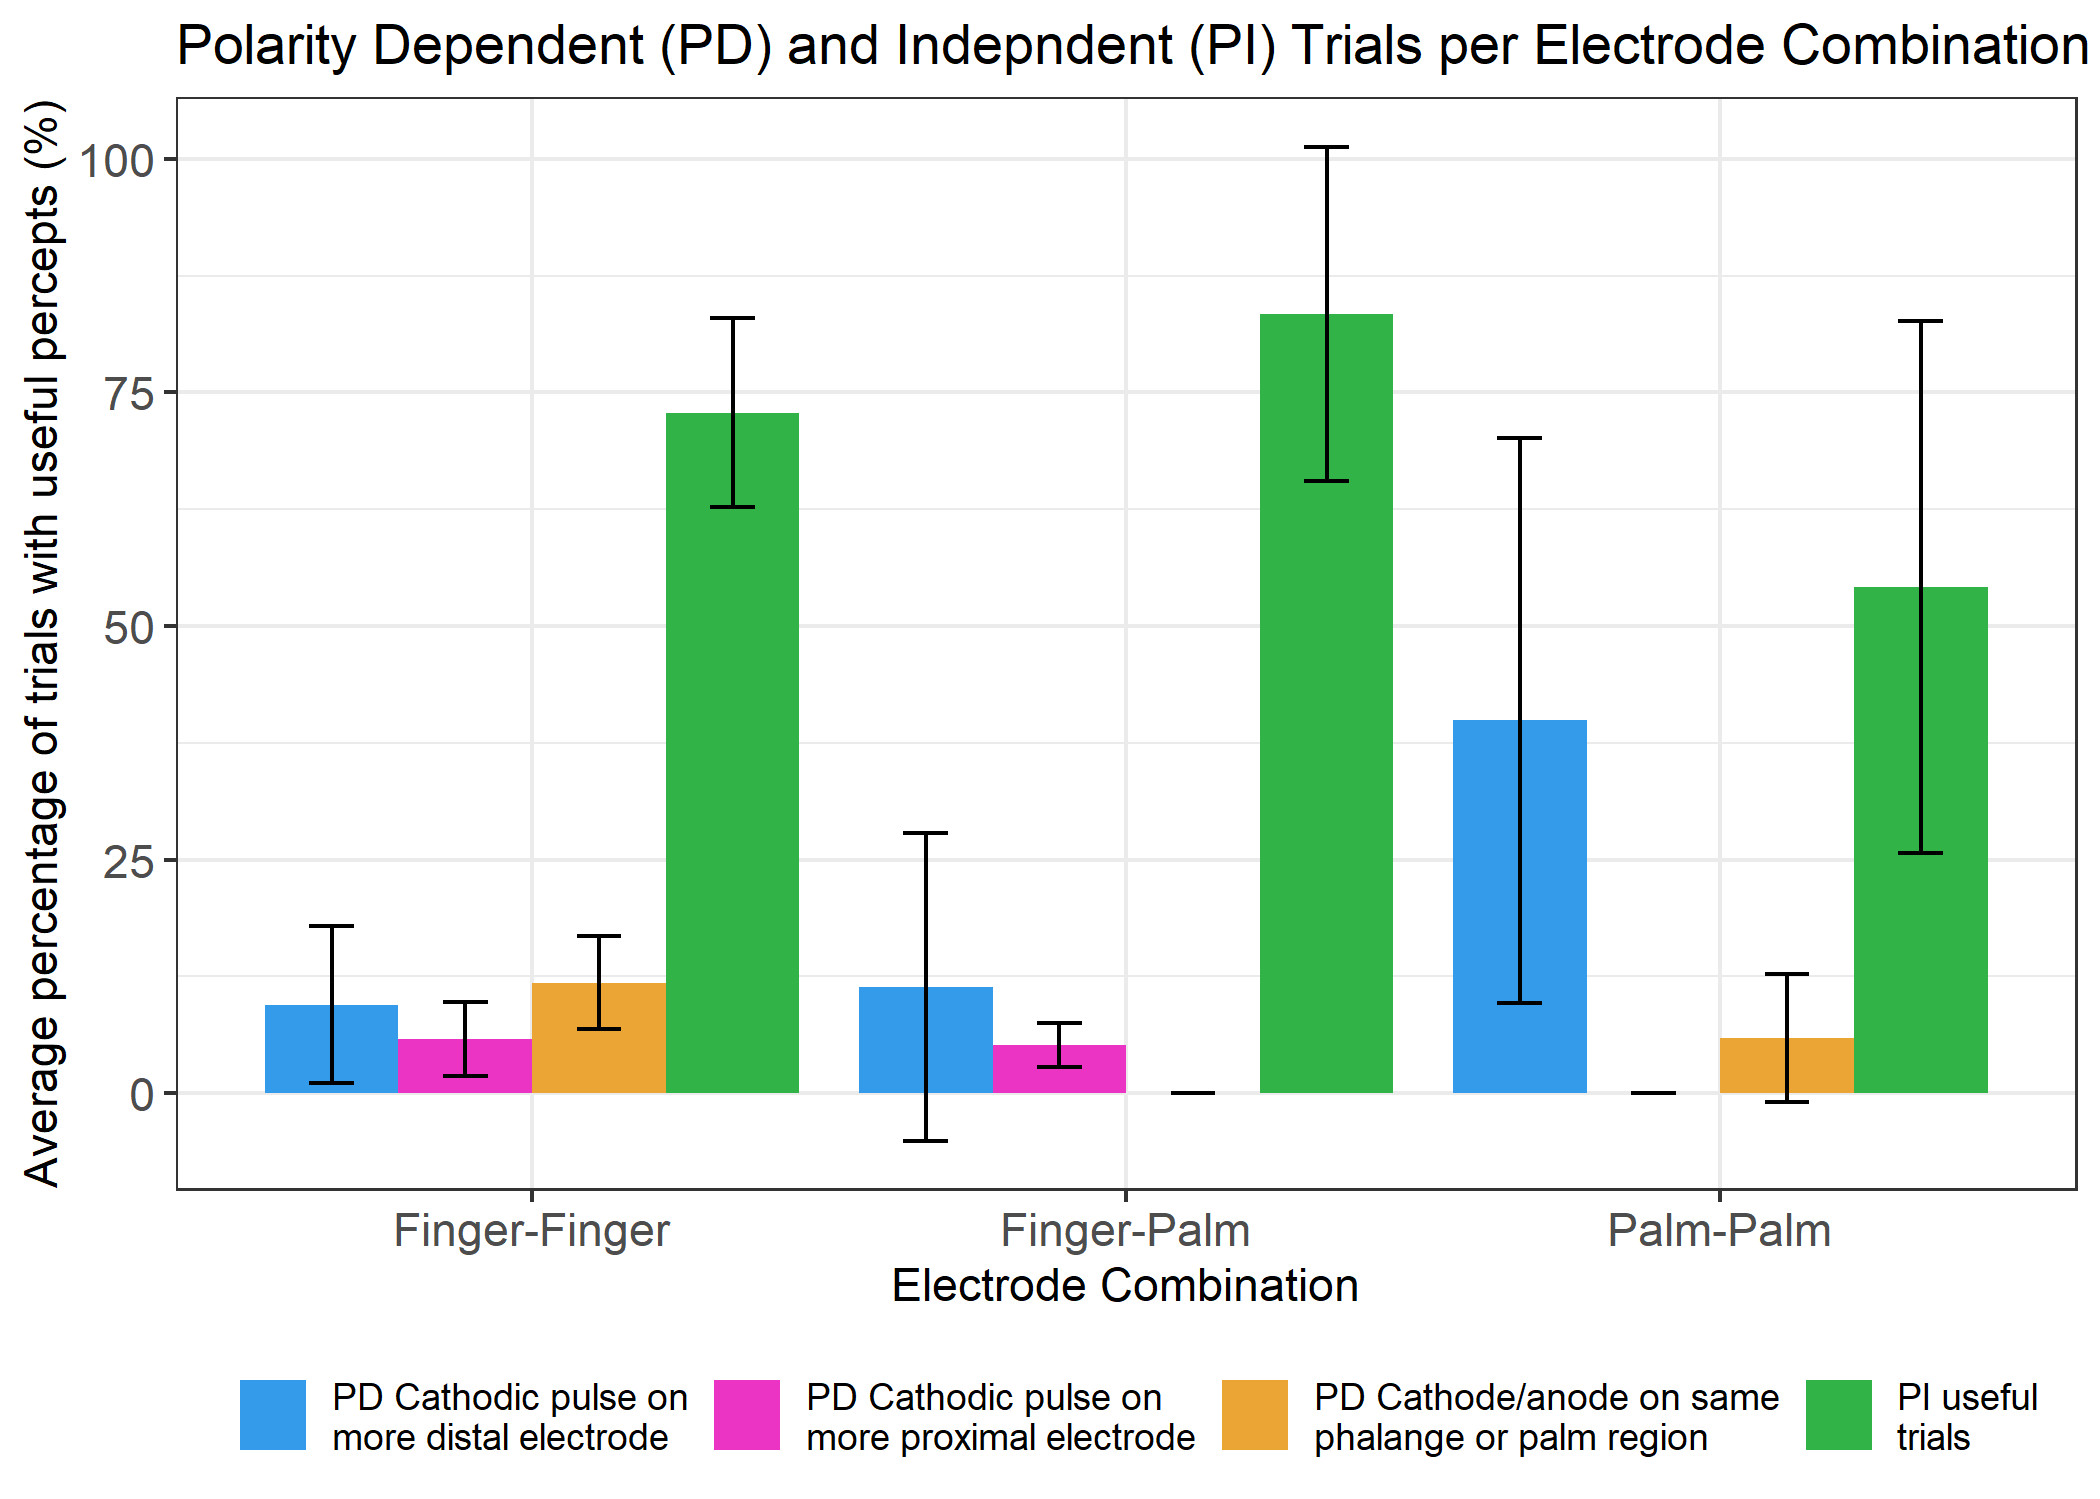
\includegraphics[trim={0cm 0cm 0cm 0cm},width=0.5\textwidth,clip]{fig/explo_res_polarityComb.jpg}
    \label{fig:explo_polarityComb}}
    \subfloat[]{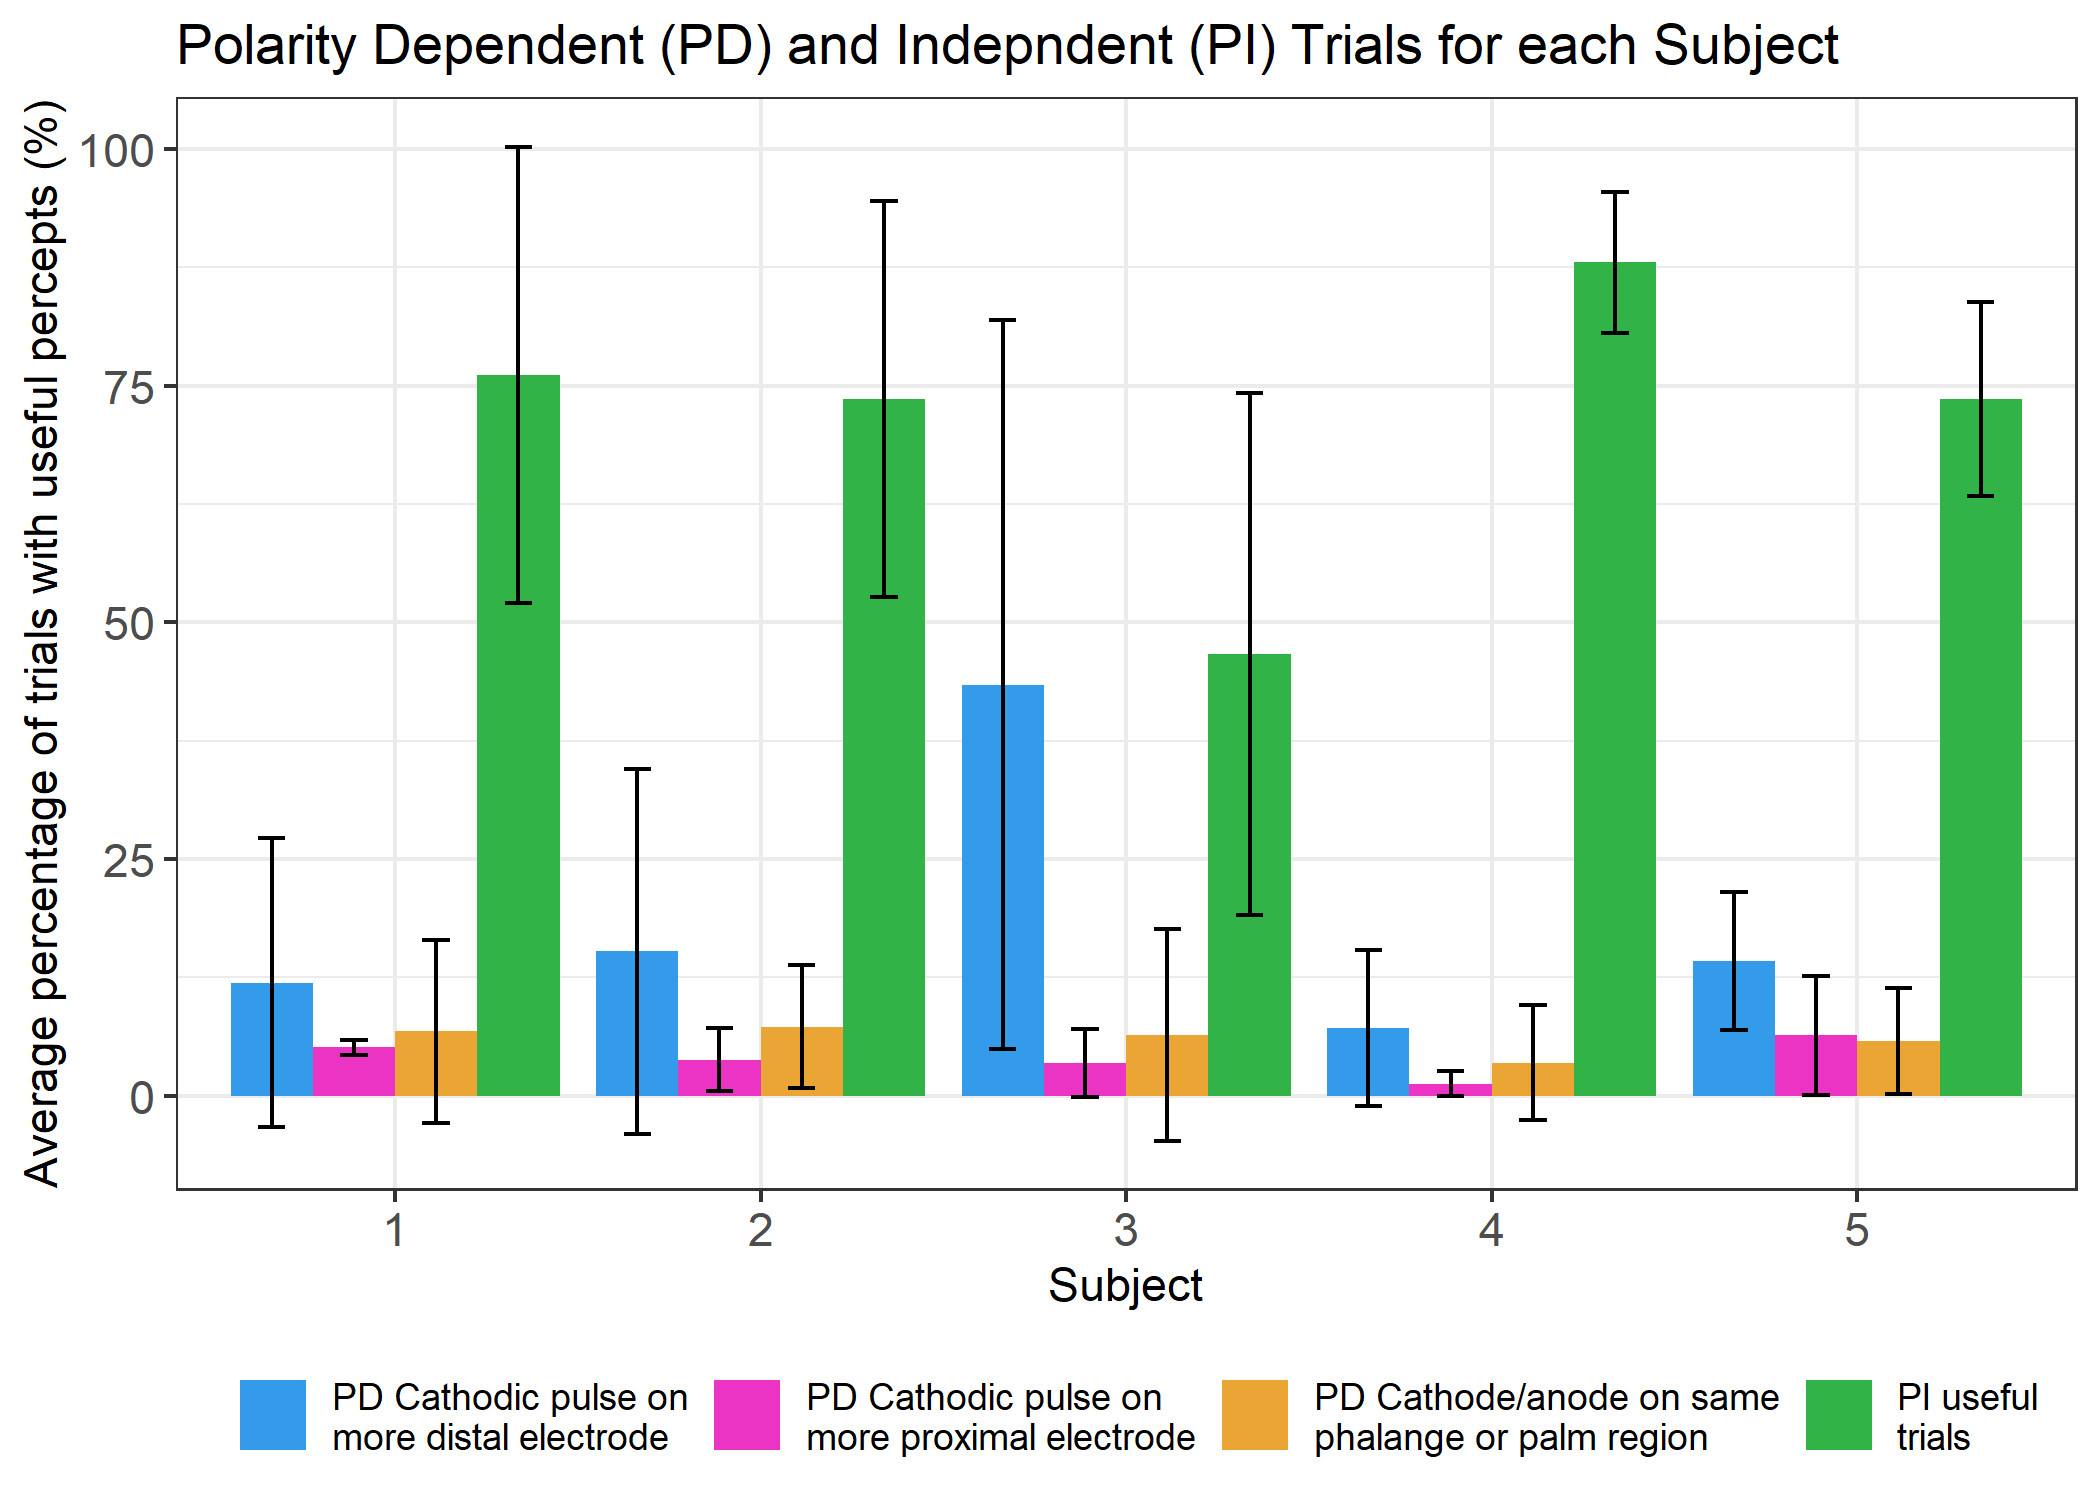
\includegraphics[trim={0cm 0cm 0cm 0cm},clip, width=0.5\textwidth]{fig/explo_res_polaritySub.jpg}
    \label{fig:explo_polaritySub}}
    \caption{The polarity dependent average percentage and standard deviation relative to the total useful trials for (\ref{fig:explo_polarityComb}) each electrode combination averaged across subjects (n=280 finger-finger, n=480 finger-palm, n=150 palm-palm) and (\ref{fig:explo_polaritySub}) for each subject averaged across electrode combinations (n=182 per subject). The legend specifies the polarity configuration and the relative position of electrodes to each other. Orange refers to conditions where both electrodes were equidistant from the wrist per Fig. \ref{fig:electrodes_positions}, such as PP-PA or PP1-PA1.
    }
    \label{fig:explo_polarity}
\end{figure*}

\subsection{Experiment Two: Methods}

\paragraph{Participants and Study Visits:} Twelve participants were recruited, but one participant did not complete the study. The remaining eleven participants (three female, eight male; age 30 $\pm$ 14 years) participated in one three-hour session, followed by two 2.5-hour sessions. All participants provided written informed consent to participate in these experiments, which were approved by the Metro Health System Institutional Review Board. Sensation locations were evaluated for nine electrode combinations.

\paragraph{Selection of the Nine Electrode Combinations:}
During Experiment One, two participants reported during multiple trials that they perceived sensations located near the electrode positions on the palm. These sensations were outside the index finger area, so the participants were instructed to classify all trials with sensations located on the palm as not useful. Similar instances could have affected useful rates for combinations with electrodes on the palm. We hypothesized that return electrode size, inter-electrode distance, and distance from underlying nerves can increase stimulation threshold selectively at the return electrode size, so we replaced the one of the top three return electrodes with a five centimeter electrode placed over the olecranon process (elbow electrode). The nine electrode combinations for Experiment Two consisted of all the possible combinations between three finger locations (IA, IL, PL) and three non-finger locations (PA1, PP1, Elbow). The electrode positions were selected based on the three most useful finger electrodes and three most useful palm electrodes, with the elbow electrode replacing PA2 (Fig. \ref{fig:explo_elec_comb}).

Nine electrode combinations were evaluated: IA-PA1, IL-PA1, PL-PA1, IA-PP1, IL-PP1, PL-PP1, IA-Elbow, IL-Elbow, PL-Elbow. Only one polarity orientation was investigated for each combination, in which the active electrode was the most distal electrode position. This polarity was chosen because Fig. \ref{fig:explo_polarity} showed that the majority of the trials in Experiment One did not have polarity dependence, and when they did, they were more likely to be reported as useful when the distal electrode was the active electrode.

\paragraph{Preparation:} To ensure the electrode positions were consistent with those in Experiment One and repeatable across sessions, they were identified and marked using the same process described in Sec. \ref{sec:PossibleElectrodes}.

\paragraph{Parameter Search:} Sensation locations were evaluated at two different pulse widths, perception threshold and maximum comfortable limit. The pulse widths corresponding to perception threshold and maximum comfortable limit were recorded at five different pulse amplitudes (2, 3, 7, 15, and 30 mA). 

To find the perception threshold, parameter estimation by sequential testing (PEST) methodology was used to reduce participant sensory response variability \cite{slopsema_natural_2018, forst_surface_2015}. The PEST method consists of starting with a subthreshold stimulus and increasing the pulse width by a fixed step size in an ascending staircase until a sensation is reported, followed by decreasing pulse width in a descending staircase until the sensation disappears. This process was repeated until five reversals were recorded. With each reversal, the step size decreases until 1 $\mu$s step size is reached (the minimum pulse width step size for the stimulator). The pulse width step sizes used on each reversal were 20, 10¸ 5, 2, and 1 $\mu$s.

The maximum comfortable limit was defined as the maximum pulse width before sensation becomes uncomfortable, which was defined as the feeling of slight pain or physical discomfort. Furthermore, participants were instructed not to confuse uncomfortable with unnatural because this experiment was not intended to evaluate sensation quality or naturalness. In addition, participants were instructed not to confuse intensity with the level of uncomfortable sensations, because some sensations could be strong but still comfortable, while others may be very weak but uncomfortable. To find this threshold, the participant increased pulse width by one $\mu$s using a mouse scroll wheel until sensation became uncomfortable. The participant then immediately decreased pulse width until the sensation was comfortable again. There were no reversals on this process to minimize re-exposing participants to uncomfortable sensations. 

\paragraph{Sensation Location Evaluation:} After determining the stimulation pulse widths associated with perception threshold and the maximum comfortable limit at each of the five pulse amplitudes, the pulse amplitude value with the highest dynamic range ($PW_{\textrm{max}} - PW_{\textrm{perception}}$) was selected for further evaluation. The perception threshold and maximum comfortable limit were re-evaluated at this selected pulse amplitude prior to further experimentation, because changes in thresholds over a short time were observed during the exploratory trials in Experiment One. The perception threshold and maximum comfortable limit were each evaluated with a psychometric intensity test (PIT) form (see and example in Fig. \ref{fig:s42}) \cite{tan_neural_2014}. In each test, the user reported the location of the sensation by coloring in an outlined illustration of a hand using up to five different colors to report up to five different sensation intensities.

To analyze sensation locations reported by subjects, the sensation location centroid and borders were calculated. Due to discontinuities in the x-axis between fingers and the complex three-dimensionality of the fingers, 2D metrics like centroids and bounds were not suitable for evaluating sensation patterns on the x-axis as drawn on the PIT forms. Therefore, the y-axis patters were evaluated numerically, and the x-axis patterns were valuated visually. To analyze the patterns on the y-axis, the vertical centroid was calculated by averaging the y-axis distance of every colored pixel with reference to the center of the proximal phalange, which was the most proximal active electrode position. The proximal and distal bounds were the most distal and proximal aspects of each trial's sensation location. Their y-axis distances were calculated the same way as the vertical centroid. To give a numerical summary across different subjects, the vertical centroid, proximal bound, and distal bound were averaged across all subjects.

To evaluate the patterns of the perceived sensations along the x-axis, the PIT forms from different participants were superimposed with the other participants for that same electrode combination. Superimposing all percepts regardless of reported intensity might be misleading since a sensation in the desired place might have been reported, but its intensity might have been minimal while the most intense sensations would be on a proximal area of the finger, the palm, or another finger. Two superimposed outputs were created in order to show the patterns for all the sensations reported, as well as only the sensations that the participant reported as the most intense sensation during each trial.

\paragraph{Data Analysis:}
To analyze the effect of stimulation intensity on the sensation location, the various metrics used to analyze sensation location (centroid, most distal sensation, most proximal sensation, and envelope size) were average across all subjects and electrode combinations. The data was assessed for normality using a Q-Q plot and histograms, but the data did not fit a normal distribution. Therefore, a non-parametric paired difference test, Wilcox signed-rank test, was used to evaluate if stimulation intensity affected each of the different metrics. To evaluate if electrode combinations had an effect in sensation location metrics at different stimulation intensities, a non-parametric repeated measure test, Friedmann’s test, was used. 

\subsection{Experiment Two: Results}
\begin{figure}[t]
  \centering
  \subfloat[]{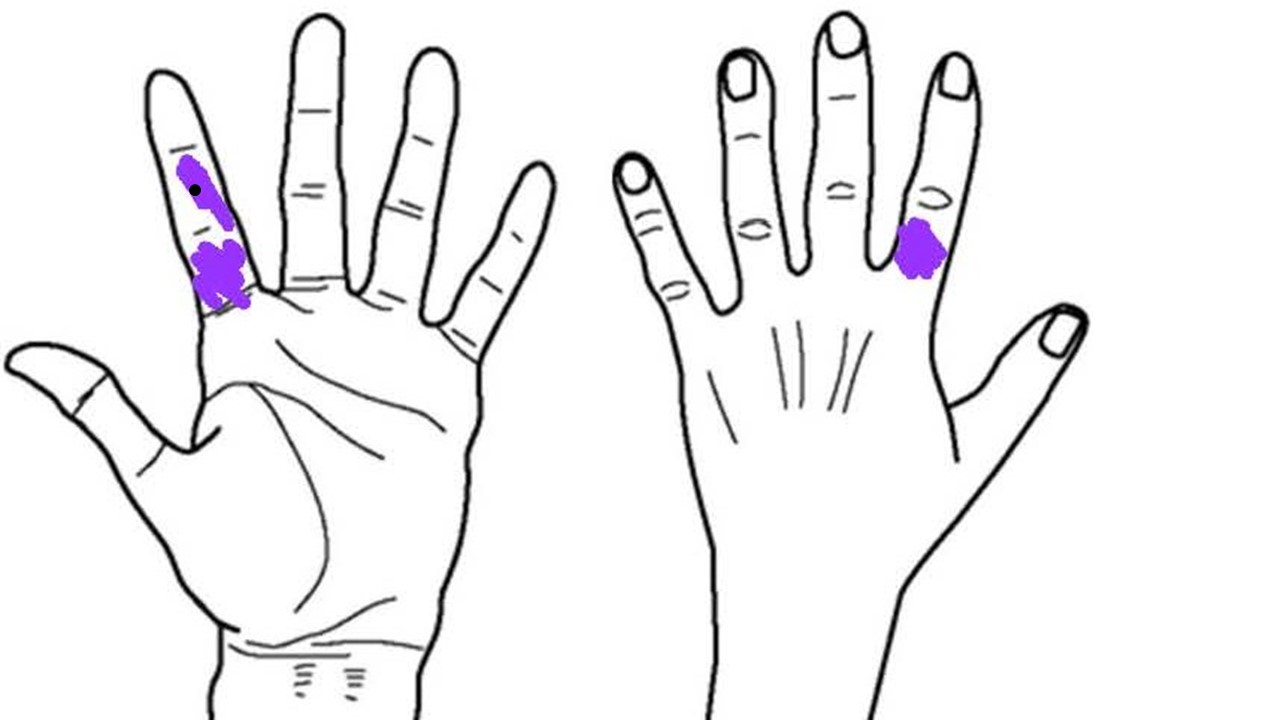
\includegraphics[width=0.25\textwidth, trim={0cm 0cm 5cm 0cm},clip]{fig/S0461.jpg}
  \label{fig:s41}}
  \subfloat[]{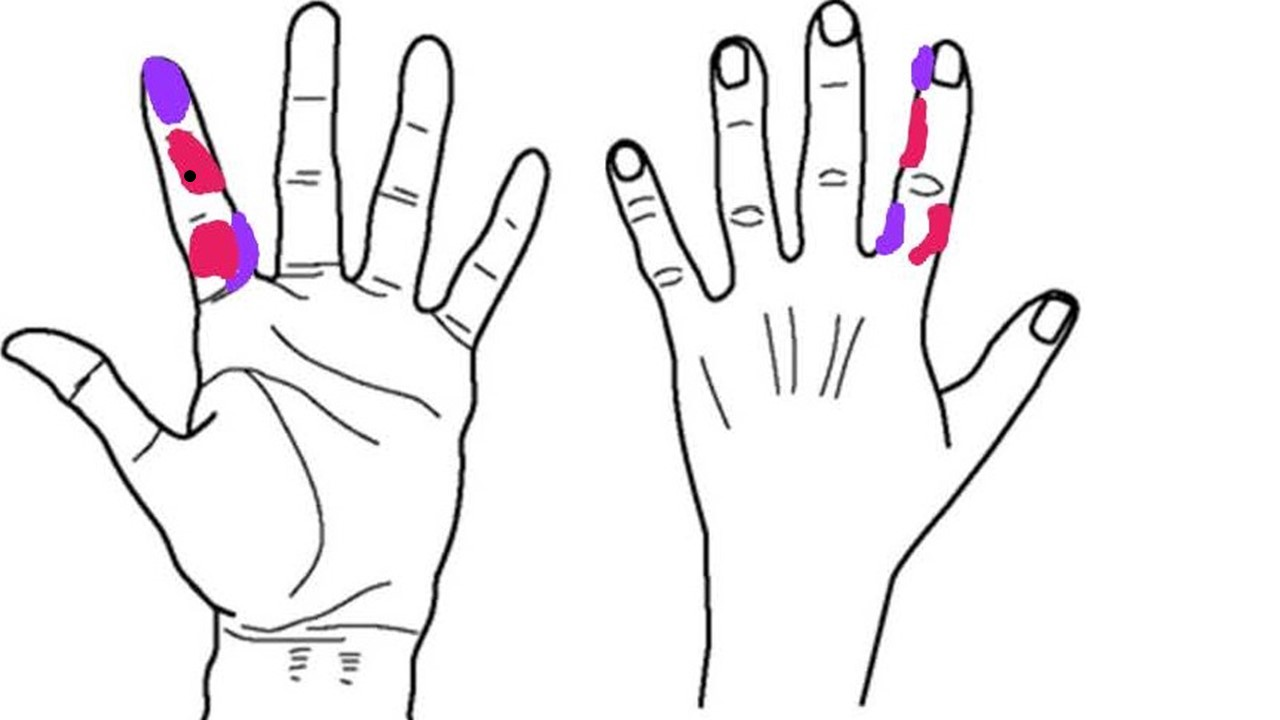
\includegraphics[width=0.25\textwidth, trim={0cm 0cm 5cm 0cm},clip]{fig/S0462.jpg}
  \label{fig:s42}}
  \caption{A single participant's (S4) psychometric intensity test form showing sensation locations for the perception threshold (\ref{fig:s41}), and the maximum comfortable limit (\ref{fig:s42}) when the active electrode was in the IA (black dot) and the return electrode was in the elbow. Purple represents the most intense percept, and pink the next most intense percept. On average, participants reported two different intensities, and the maximum number of reported intensities per trial were three.}
  \label{fig:s4}
\end{figure}

\begin{figure}[b]
  \centering
  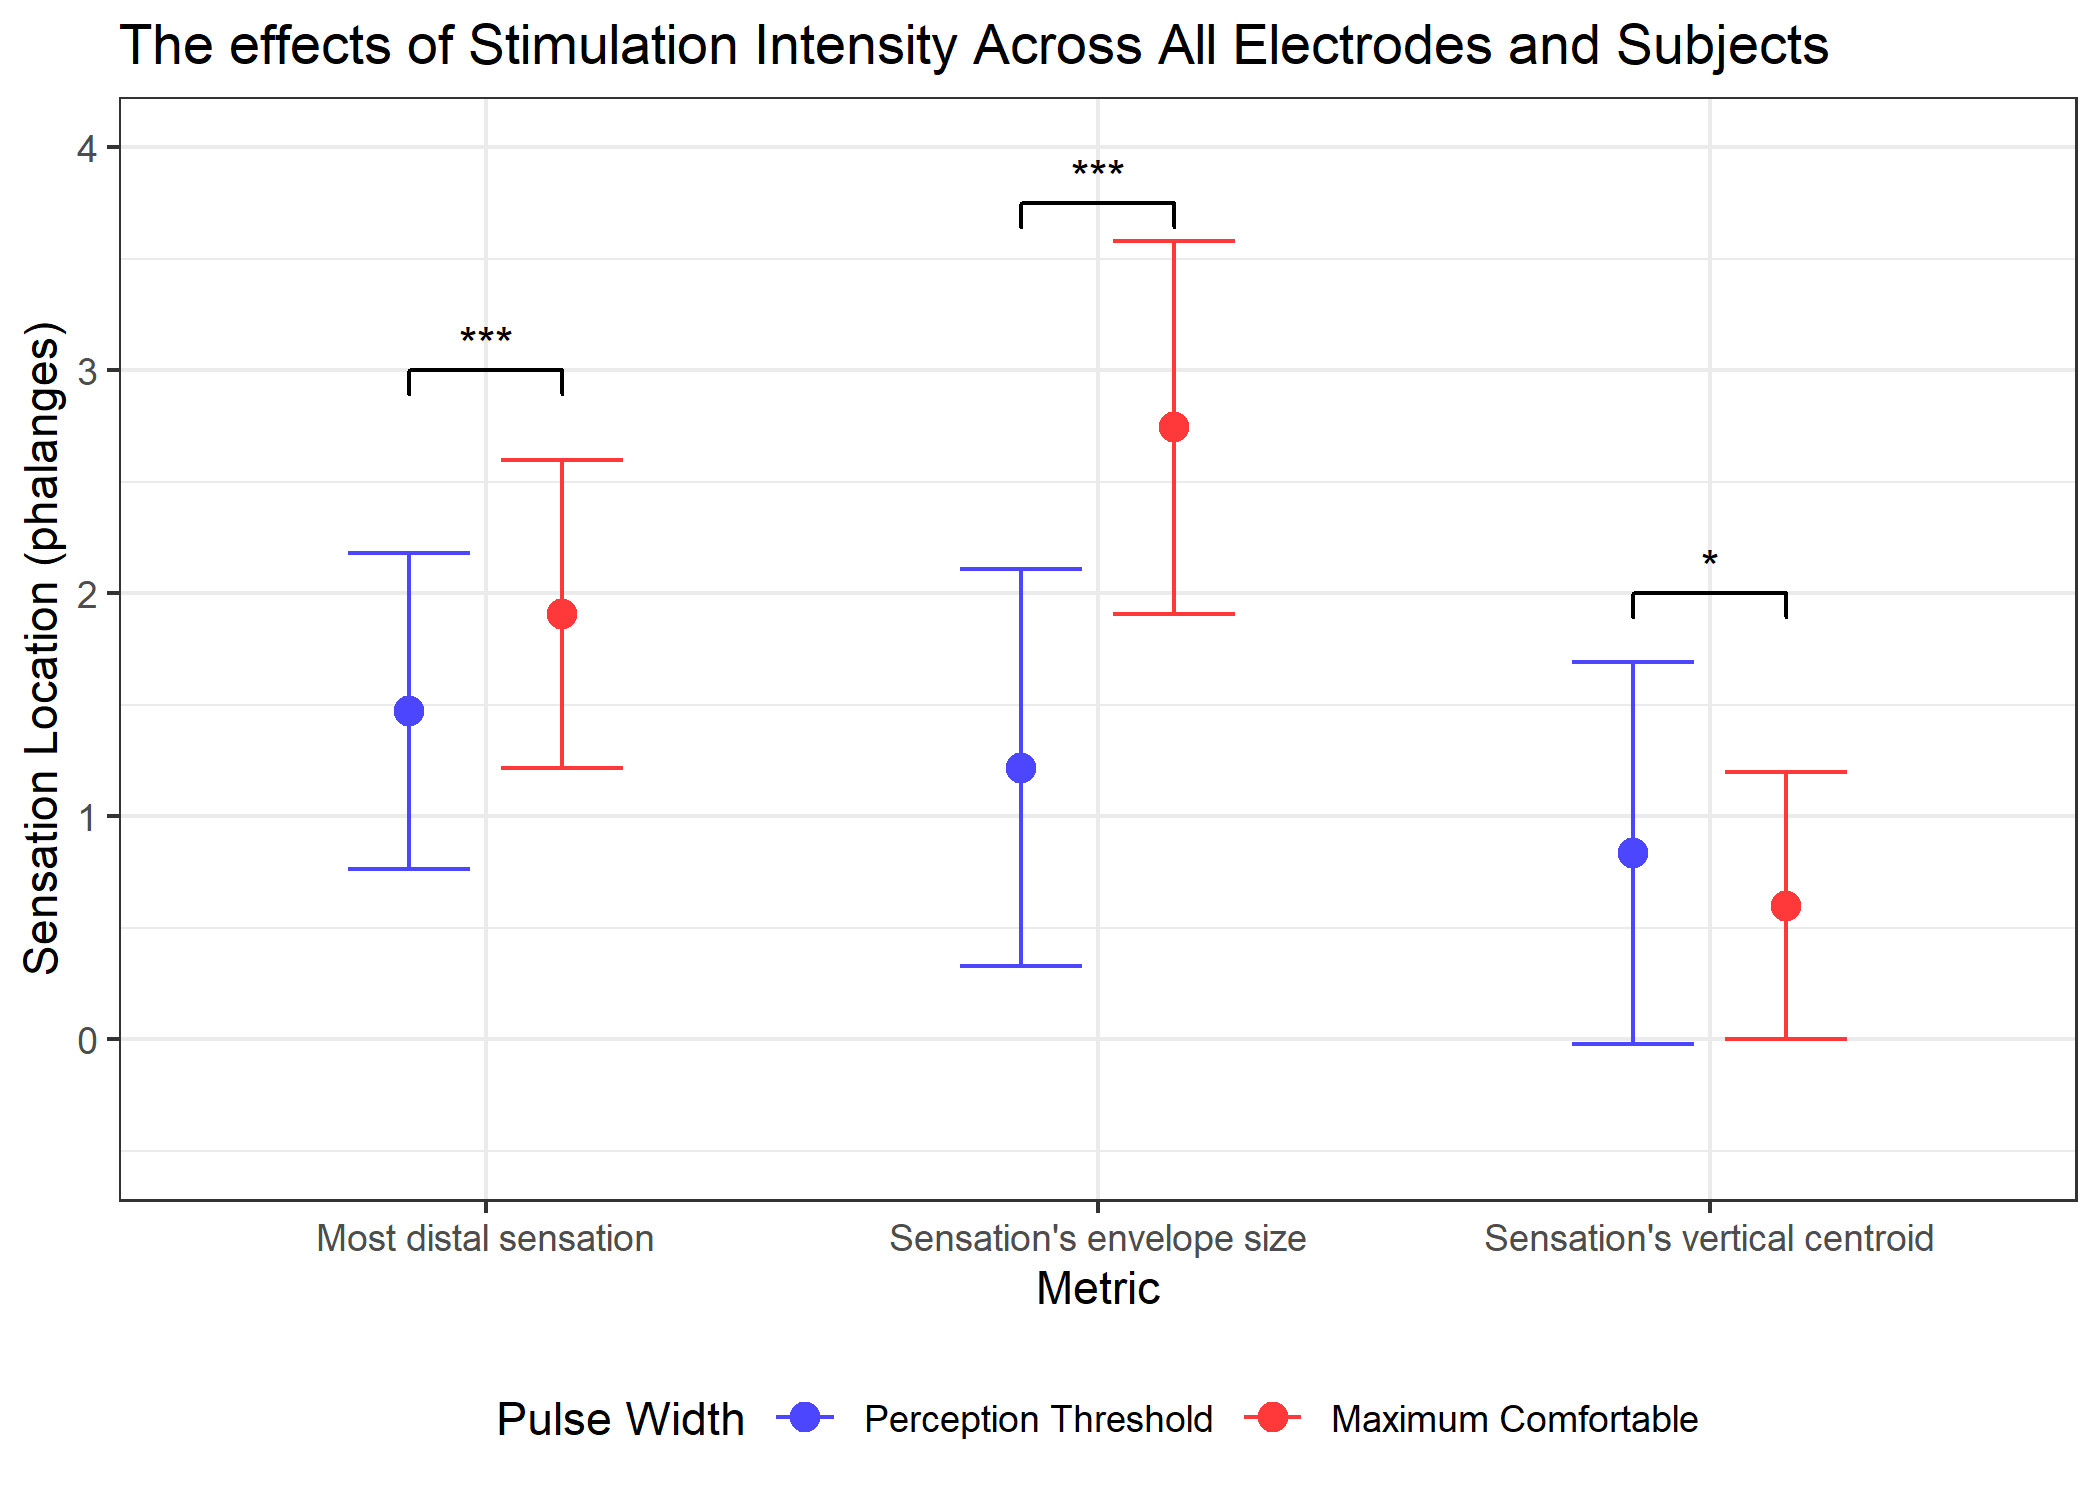
\includegraphics[width=0.5\textwidth,trim={0cm 0.5cm 0cm 0cm},clip]{fig/Stats_All_Envelopes.jpg}
  \caption{Blue represents percepts reported at the perception threshold pulse width, and red represents percepts reported at the maximum comfortable limit. The x-axis shows different metrics comparing the effect of stimulation intensity on sensation location, normalized to finger phalanges. The point denotes the mean across all electrode combinations and subjects, and the errors bars show standard deviation (n=99 per stimulation intensity on each metric). The statistical significance was calculated using Wilcoxon signed-rank test. The data separated by electrode combination is shown in Figure \ref{fig:all_cent}.}
  \label{fig:w_test_res}
\end{figure}

\paragraph{Sensation location centroids and envelopes:}
Figure \ref{fig:s4} shows an example PIT form reported by Subject 4 for the IA-elbow electrode combination, with different colors representing the intensity of perceived sensation in different areas. At the maximum comfortable limit, the perceived sensation area changed, as shown by the differences between Figures \ref{fig:s41} and  \ref{fig:s42}. This illustrates that changes in the sensation's locations could be elicited by changes in stimulation pulse width and that the sensation area can expand and move in the distal-proximal direction with greater stimulation intensity. 

We then calculated three metrics to describe the spatial extent of the perceived sensory locations. All metrics are relative to the long axis of the finger (or the y-axis). For each trial, the percept centroid is the average y-axis position, the distal boundary is the most distal y-axis position, and the proximal boundary is the proximal y-axis position (Fig. \ref{fig:s4_cent}). The distance between the proximal and distal boundaries (referred to as the envelope) increased as stimulation intensity was increased from the perception threshold to the maximum comfortable limit (Fig. \ref{fig:s4_cent}).  This increase in percept size with increasing stimulation intensity occurred for all electrode combinations, except for the PL-PA1 electrode combination. Furthermore, four of the nine electrode combinations for Subject 4 showed distally referred sensations, which we defined as when segments of the sensations were located at least one phalange away from the active electrode in the distal direction. These distally referred sensations were all located on the fingertip between 1.5 to 2.7 phalanges distal to the active electrode.

\begin{figure*}[b]
  \hspace*{-0.2cm} 
  \centering
  \subfloat[]{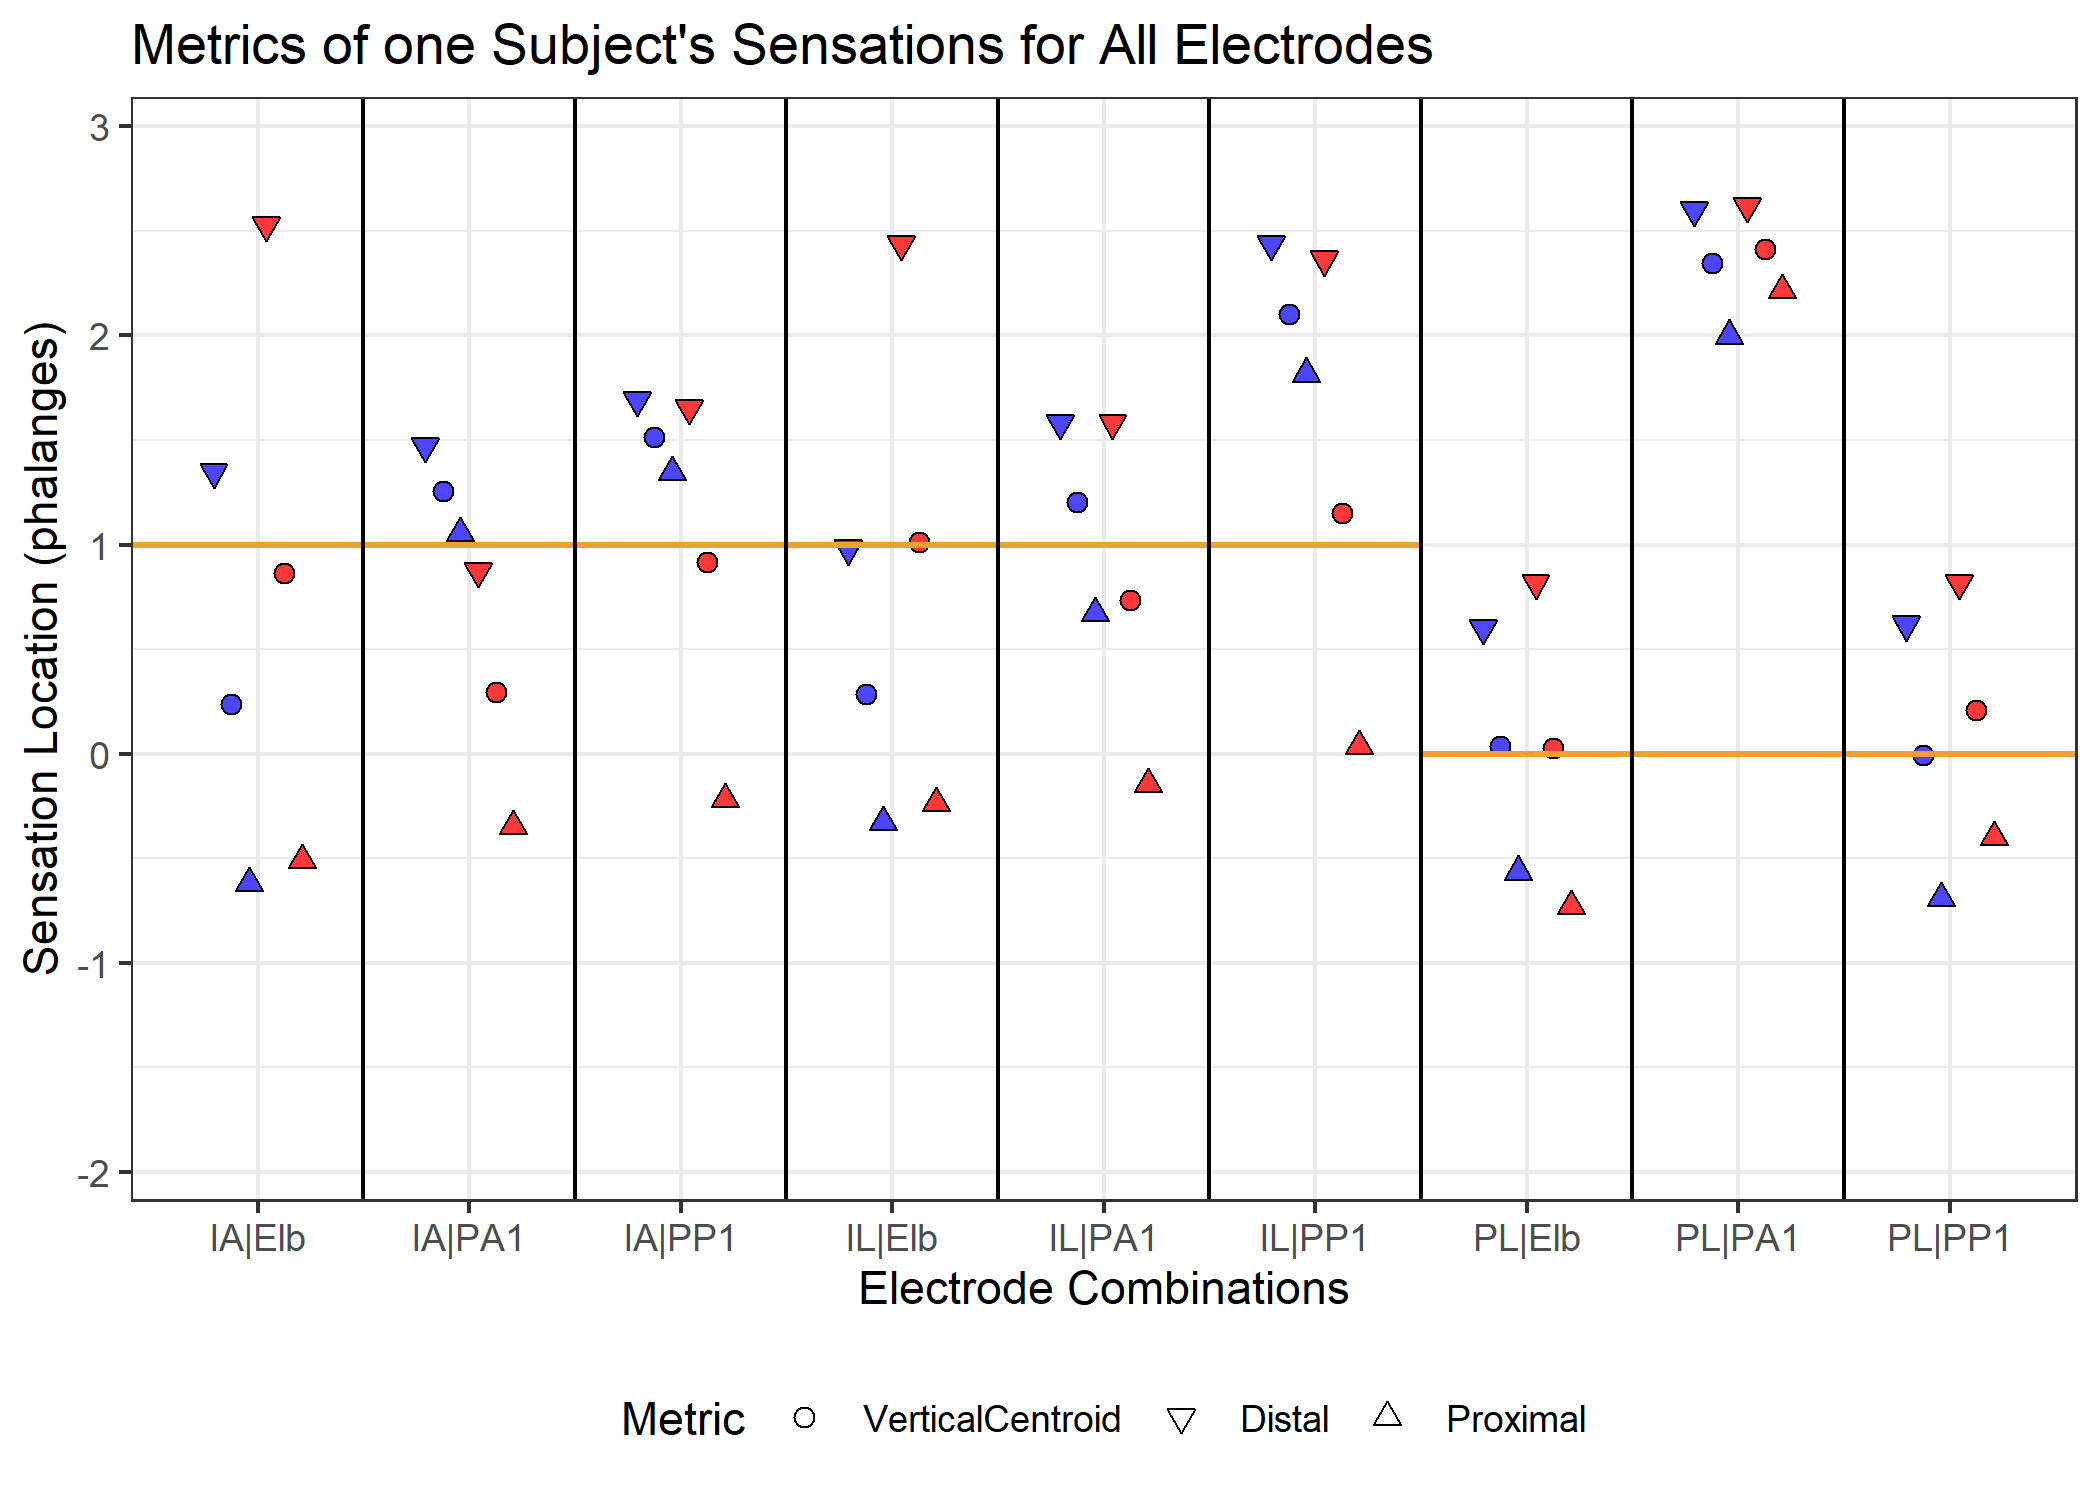
\includegraphics[width=0.42\textwidth, trim={0cm 0cm 0cm 0cm} ,clip]{fig/S4_Envelopes.jpg}
  \label{fig:s4_cent}}
   \subfloat[]{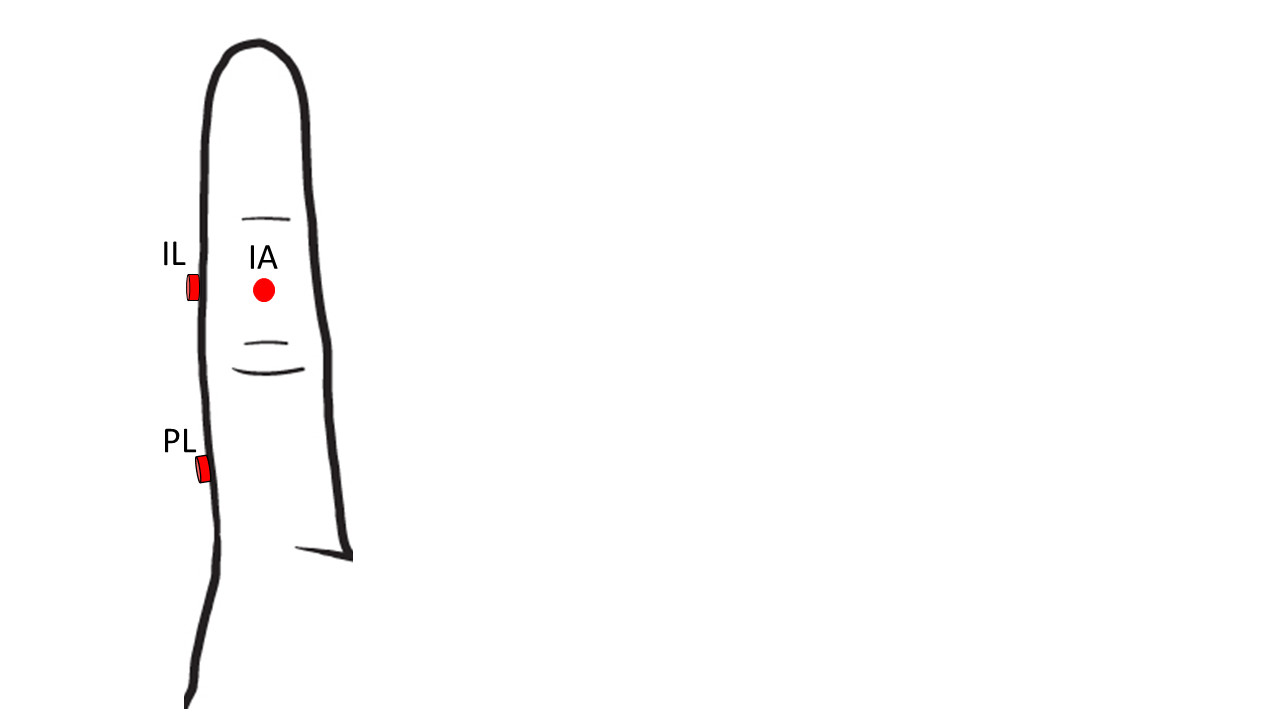
\includegraphics[width=0.045\textwidth, trim={5cm -10.2cm 25cm 1cm} ,clip]{fig/finger.jpg}
  \label{fig:finger}}
  \subfloat[]{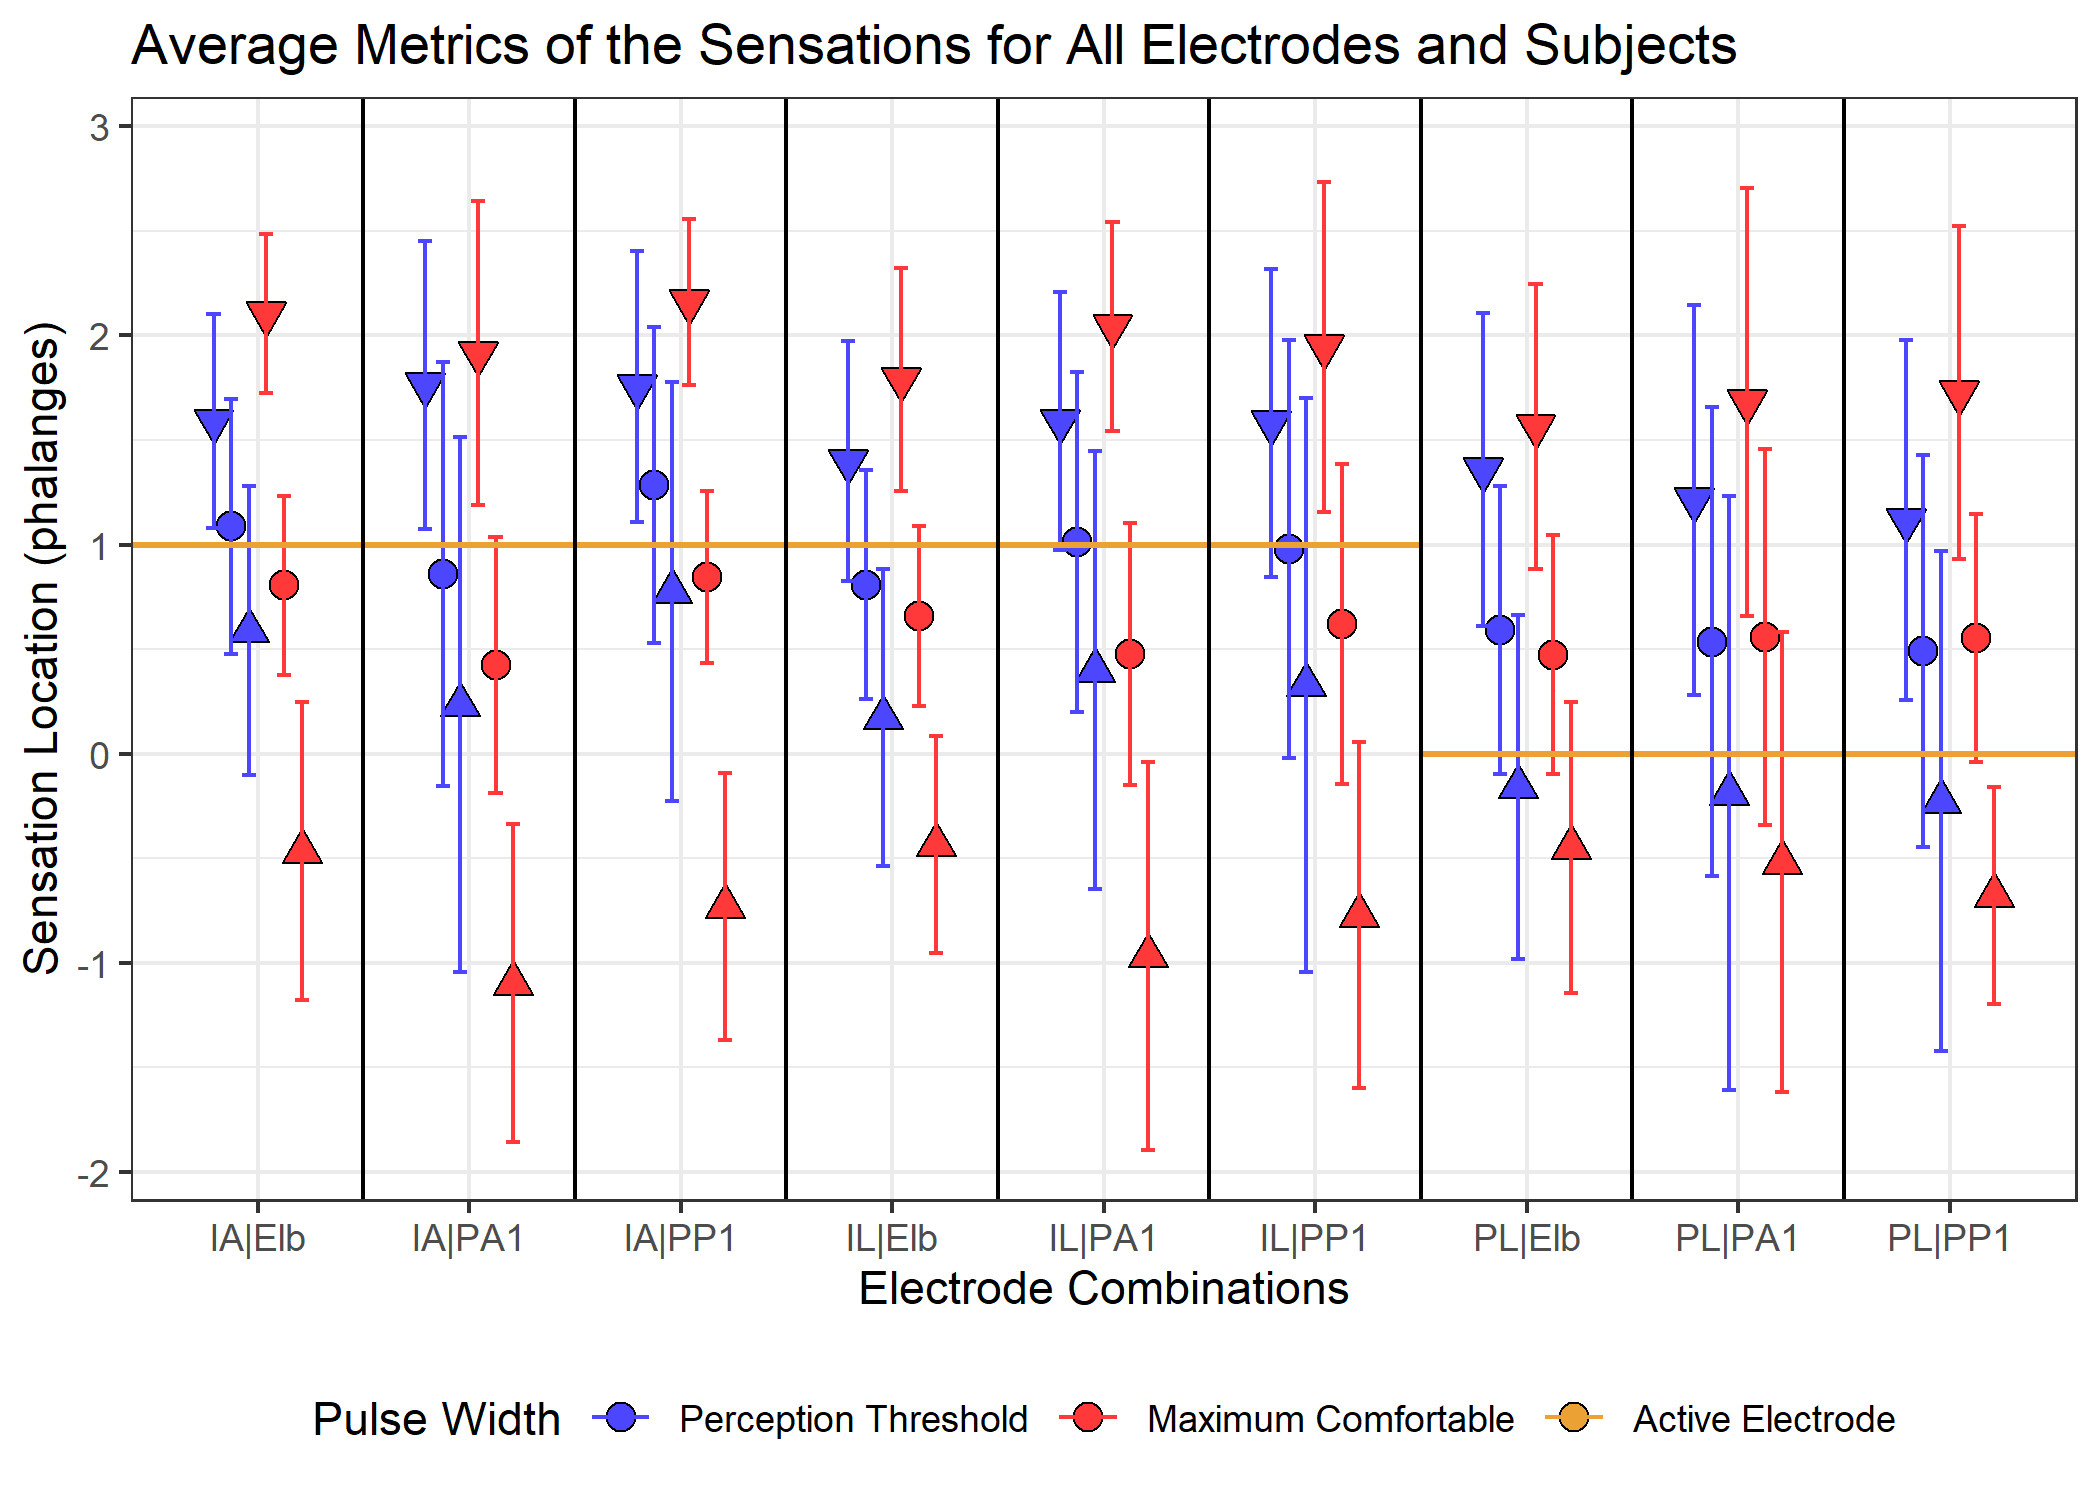
\includegraphics[width=0.42\textwidth, trim={0cm 0cm 0cm 0cm}, clip]{fig/All_Envelopes.jpg}
  \label{fig:all_cent}}
  \caption{The vertical location of the percept centroid (circle), distal boundary (downward triangle), and proximal boundary (downward triangle) in units of finger phalanges from the psychometric intensity test (PIT) forms. Blue represents percepts reported at the perception threshold pulse width, and red represents percepts reported at the maximum comfortable limit. The orange horizontal line marks the position of the active electrode for each electrode combination. (\ref{fig:s4_cent}) Shows subject 4's results, (\ref{fig:finger}) shows the PIT form's index finger that has been scaled to the axes in (a) and (c) to display the IL, IA, and PL electrode positions relative to the orange lines, and (\ref{fig:all_cent}) shows the average centroid and bounds across participants with standard deviation depicted by the error bars (n=11 per electrode combination and stimulation intensity).}
\end{figure*}

Across all participants, the centroid migrated significantly more proximally (Wilcox signed-rank test, $p=0.028$), the distal boundary migrated to a significantly more distal location (Wilcox signed-rank test, $p<0.001$), and the envelope (percept) size significantly increased (Wilcox signed-rank test, $p<0.001$) for all nine electrode combinations when stimulation intensity increased (Fig. \ref{fig:w_test_res}. In addition, electrode combinations that included the elbow for the return electrode had more proximally located proximal boundaries at the maximum comfortable limit. However, the average centroids (Friedmann's tests, $p=0.09$ for perception threshold, $p=0.71$ for maximum comfortable limit), distal boundaries (Friedmann's tests, $p=0.05$ for perception threshold, $p=0.09$ for maximum comfortable limit), and proximal boundaries (Friedmann's tests, $p=0.09$ for perception threshold, $p=0.26$ for maximum comfortable limit) were not statistically different between the nine electrode combinations.

\subsubsection{Evaluating sensation location drawings:}
Figure \ref{fig:all_hands_conf} superimposes the sensation locations drawn on the PIT forms at the maximum comfortable limit across subjects, where redder areas indicate a higher frequency of reports. Sensation locations are shown without differentiating by perceived intensity level reported within trials. The sensations reported across subjects and all electrode combinations were concentrated on the index finger (brighter colors on the index finger compared to the palm and other fingers). Only three out of the nine combinations reported sensations on another finger other than the index, and these other fingers (thumb and middle) were adjacent to the index finger somatotopically. Electrode combinations with PA1 and PP1 return electrodes also tended to generate sensations that spread to proximal areas of the palm. In contrast, electrode combinations with an elbow return caused fewer participants to experience sensations in the palm. These results agree with the differences observed between the proximal boundaries of the vertical envelopes based on electrode configuration shown in Figure \ref{fig:all_cent}. Sensations outside the index finger area were only reported by one or two participants for each electrode combination. In total, 37\% of the trials (n=99) had sensation outside the targeted finger. Electrode combinations that included an IA active electrode produced sensation locations that were approximately evenly distributed along all three phalanges of the index finger. 

\begin{figure*}
  \centering
  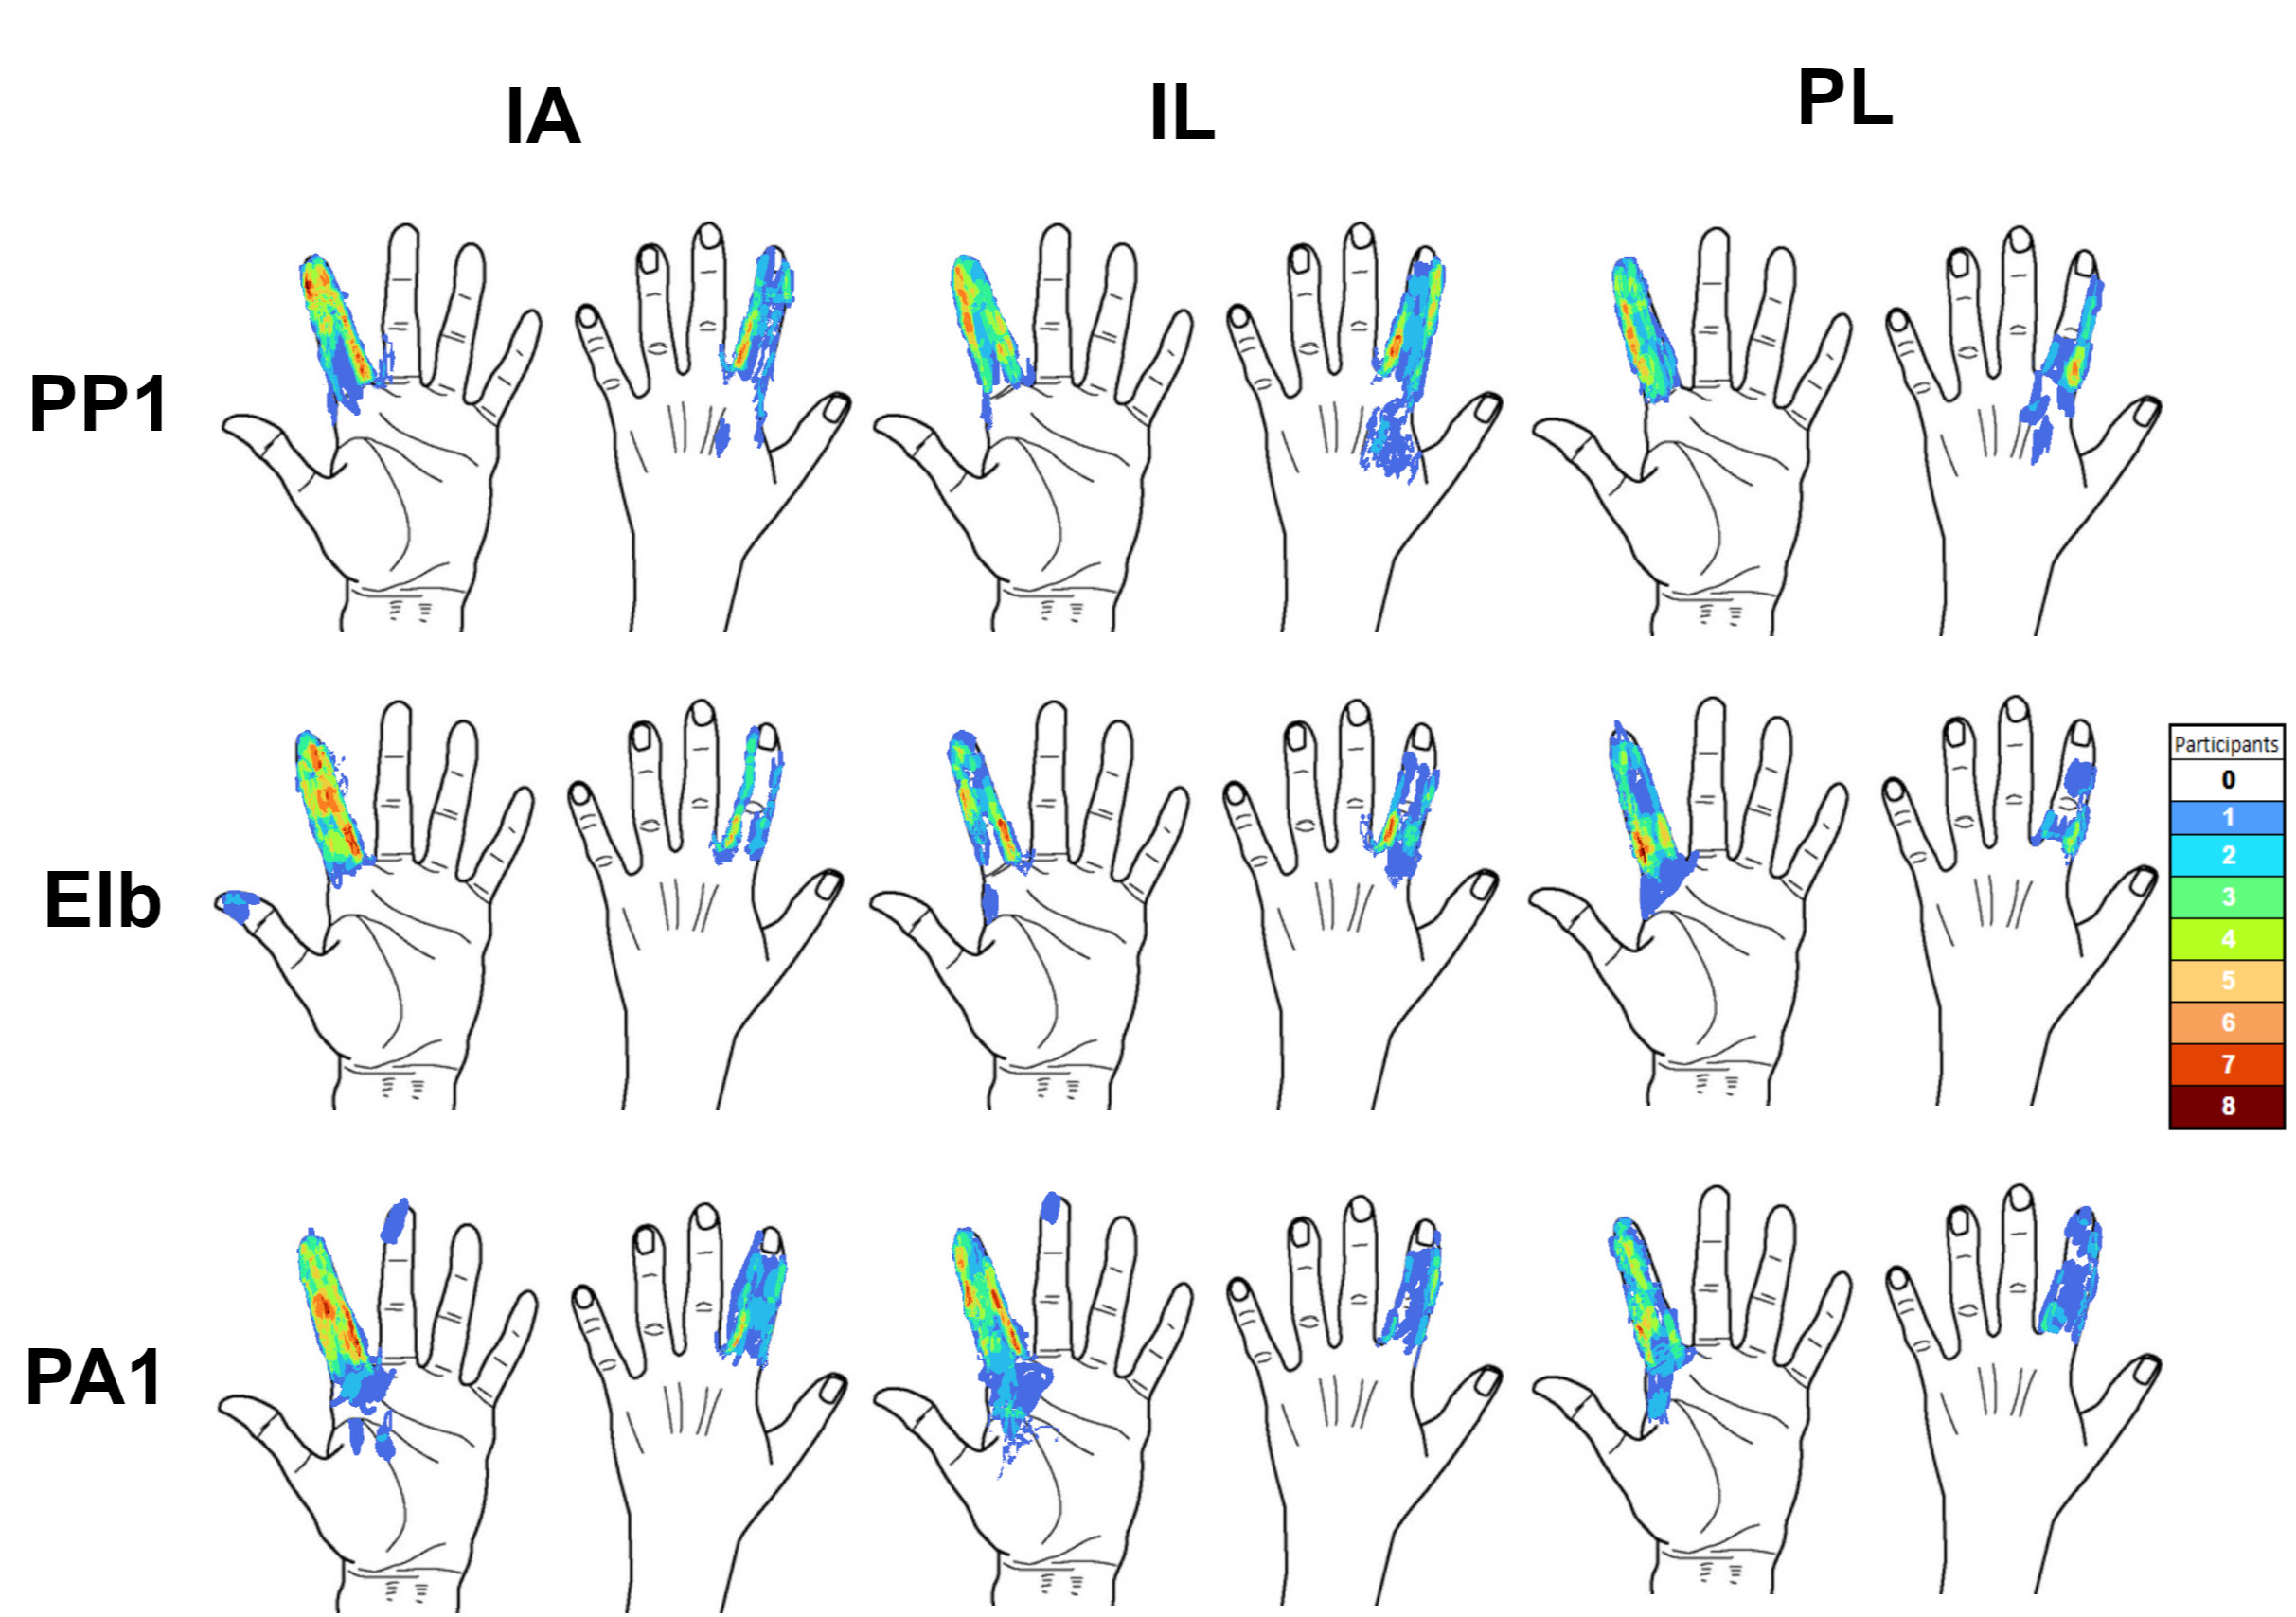
\includegraphics[width=0.9\textwidth, trim={0.5cm 0cm 0cm 0cm} ,clip]{fig/max_IMG_color.jpg}
  \caption{Percept locations reported across all eleven participants for each of the nine electrode combinations at maximum comfortable stimulation parameters. The colors represent the number of participants that experienced a sensation on a given location. These figures include \textbf{all sensations} reported, regardless of the reported intensity.}
  \label{fig:all_hands_conf}
\end{figure*}

Figure \ref{fig:all_hands_max} superimposed the reported sensation location for only the most intense sensation reported in each trial across trials and subjects. Data is shown for the trials of maximum comfortable limit only. Most of the percepts reported across all electrode combinations were focused on the index finger. Compared to Figure \ref{fig:all_cent}, the most intense sensation reported on each trial was only on the targeted finger. More importantly, all electrode combinations elicited a distally-referred sensation in the index fingertip at the most intense stimulus levels in each trial. 

\begin{figure*}
  \centering
  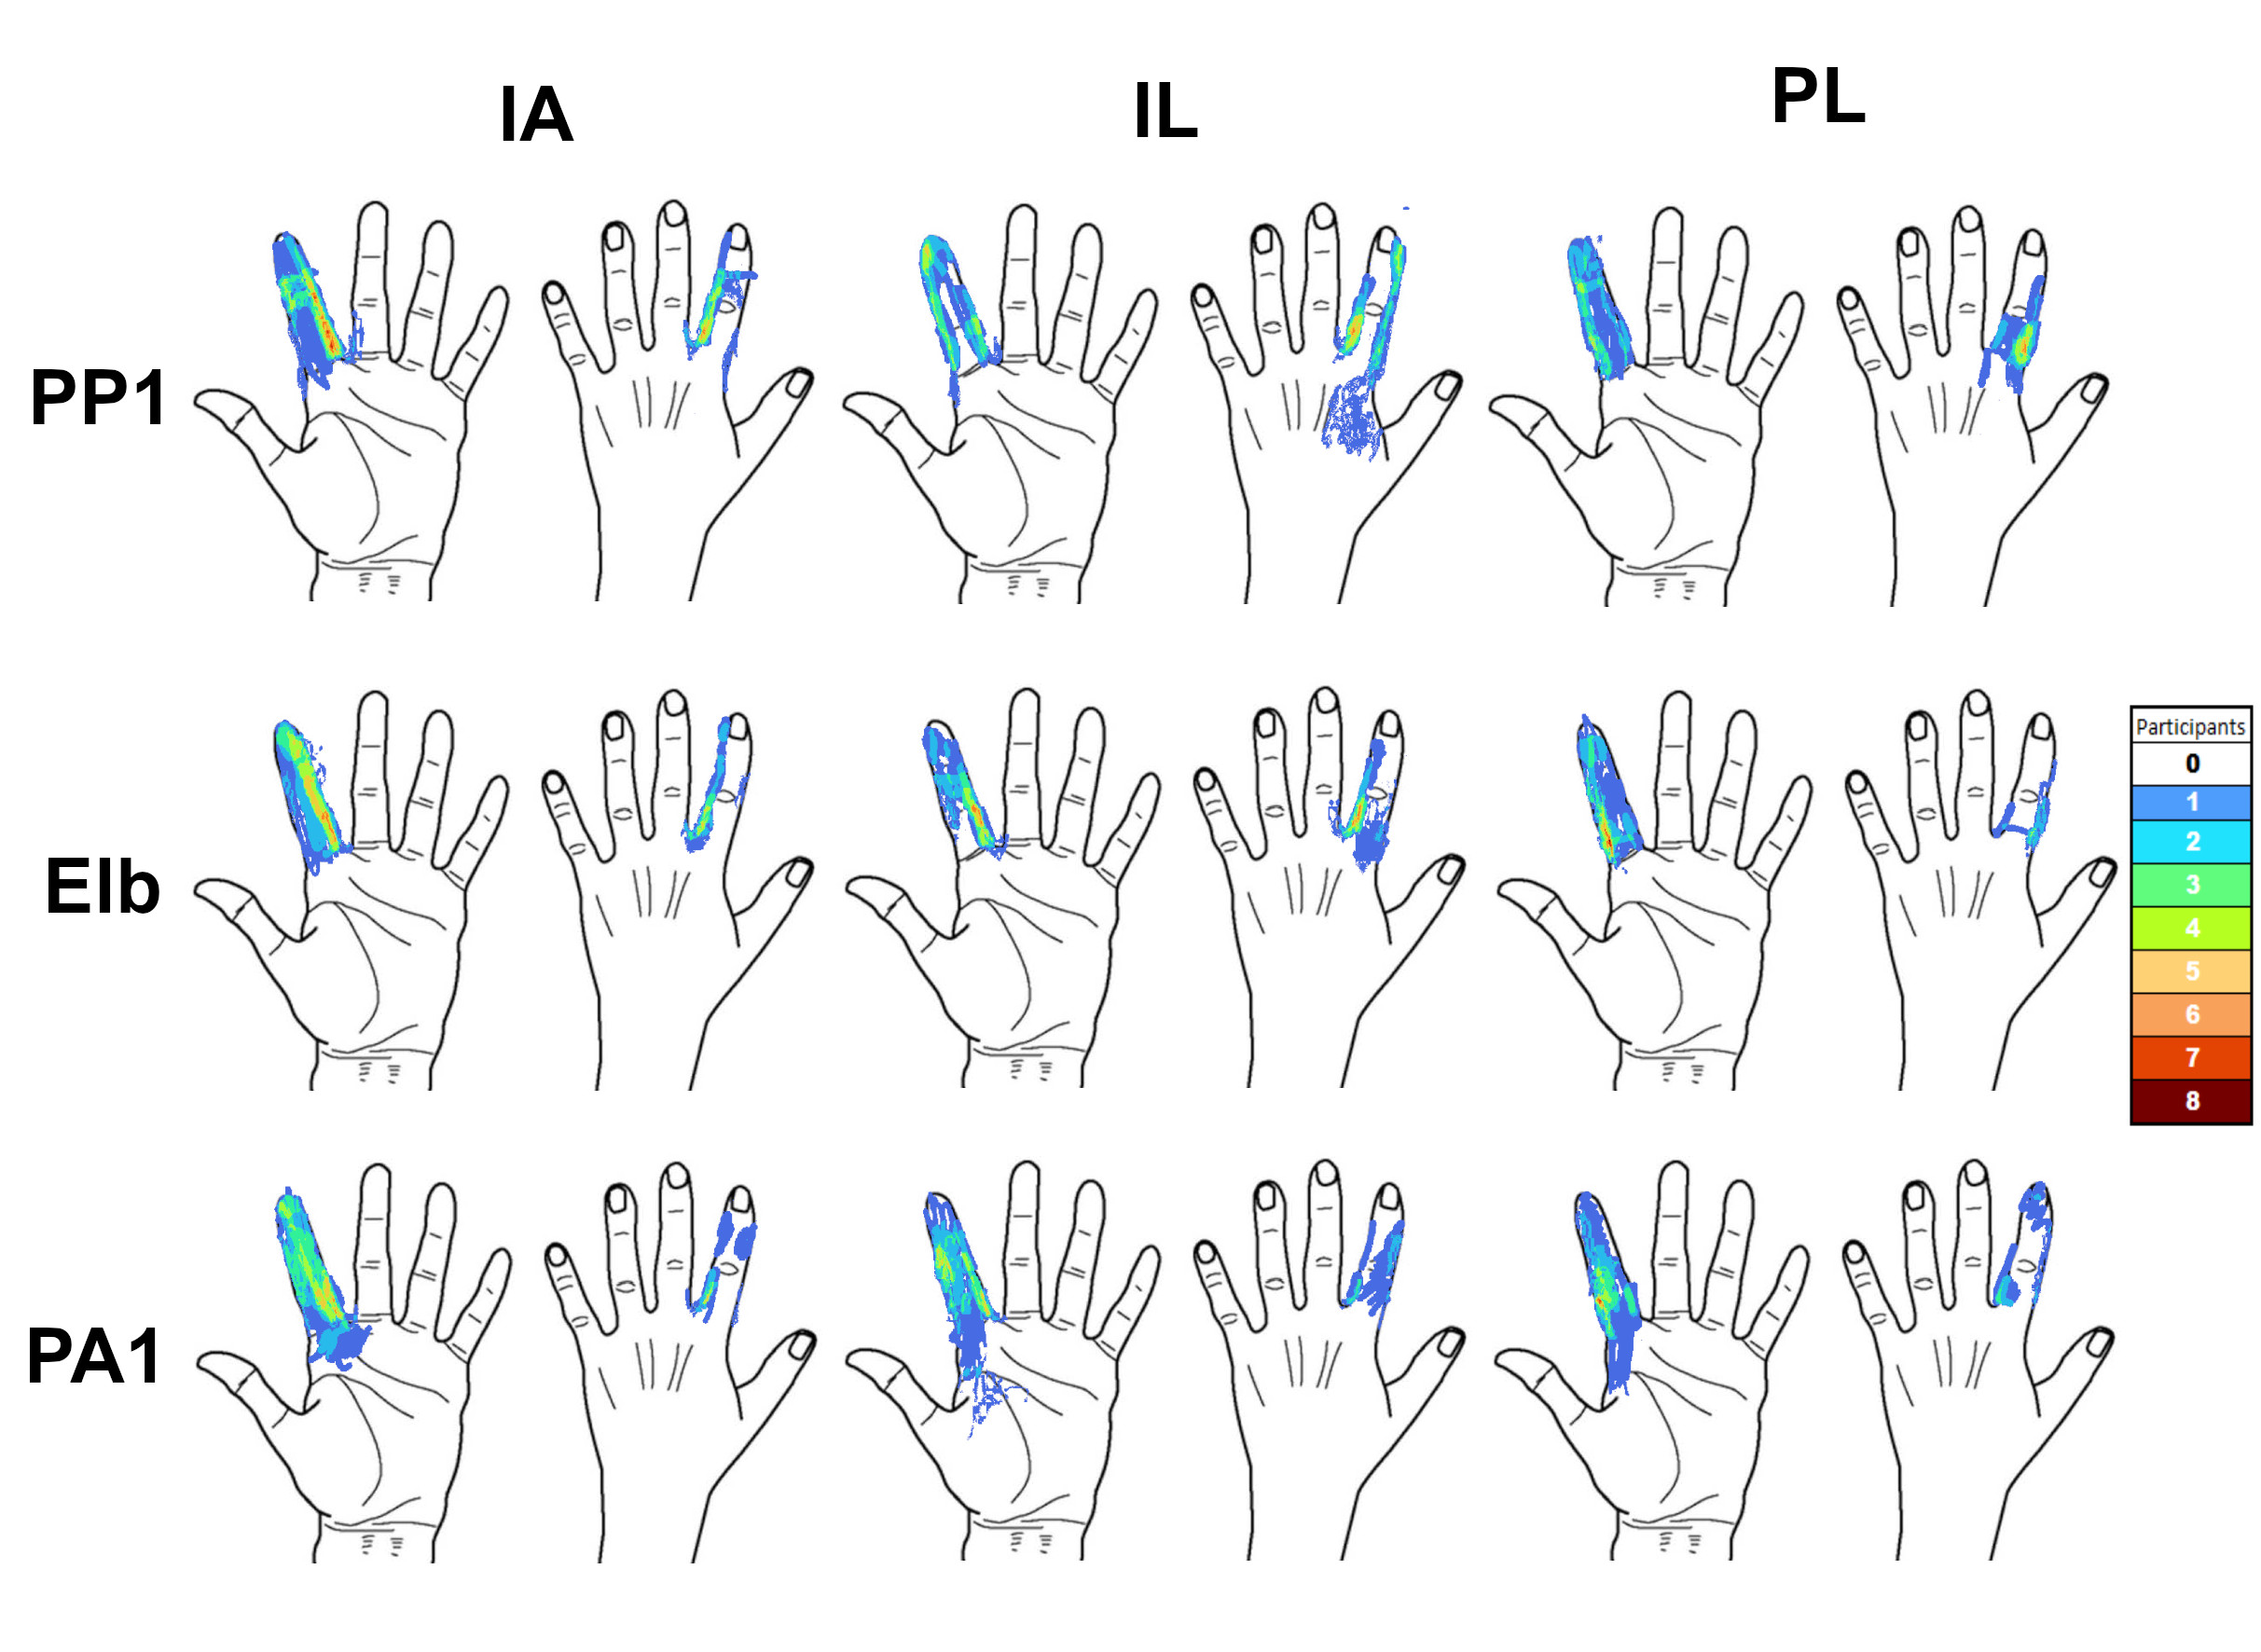
\includegraphics[width=0.9\textwidth, trim={0.5cm 0cm 0cm 0cm} ,clip]{fig/maxMax_IMG_color.jpg}
  \caption{Percept locations reported across all eleven participants for each of the nine electrode combinations at maximum comfortable stimulation parameters. The colors represent the number of participants that experienced a sensation on a given location. Only the \textbf{most intense sensation} reported in each trial are shown here.}
  \label{fig:all_hands_max}
\end{figure*}

Figure \ref{fig:distal_eva} shows which electrode combinations generated a distally-referred sensation for each participant at perception threshold, maximum comfortable limit, or both. At least one of the electrode combinations successfully generated distally-referred sensations at both perception threshold and maximum comfortable limit for all participants (Fig. \ref{fig:distal_eva}). Furthermore, some participants reported distally-referred sensations for most of the tested combinations (mean = 7.4 combinations, min = 2 combinations, max = 9 combinations).  Also, the IL-PA1 electrode combinations generated distally-referred percepts for all participants for at least one of the evaluated pulse widths. When comparing active electrodes and return electrodes, only the PL electrode position reported fewer distally-referred sensations than the other active electrodes positions. Comparing across subjects and electrode combinations, 18\% of the trials did not include a distally-referred sensation, 4\% of the trials elicited a distally-referred sensation at perception threshold only, 25\% of the trials elicited a distally-referred sensation at the maximum comfortable limit only, and 53\% of the trials elicited a distally-referred sensation at both stimulation levels (n=99). Thus, reports of distally-referred sensation were more common at the maximum comfortable limit compared to perception threshold, though reports of distally-referred sensation at both levels were by far the predominant response.

\begin{figure}
  \centering
  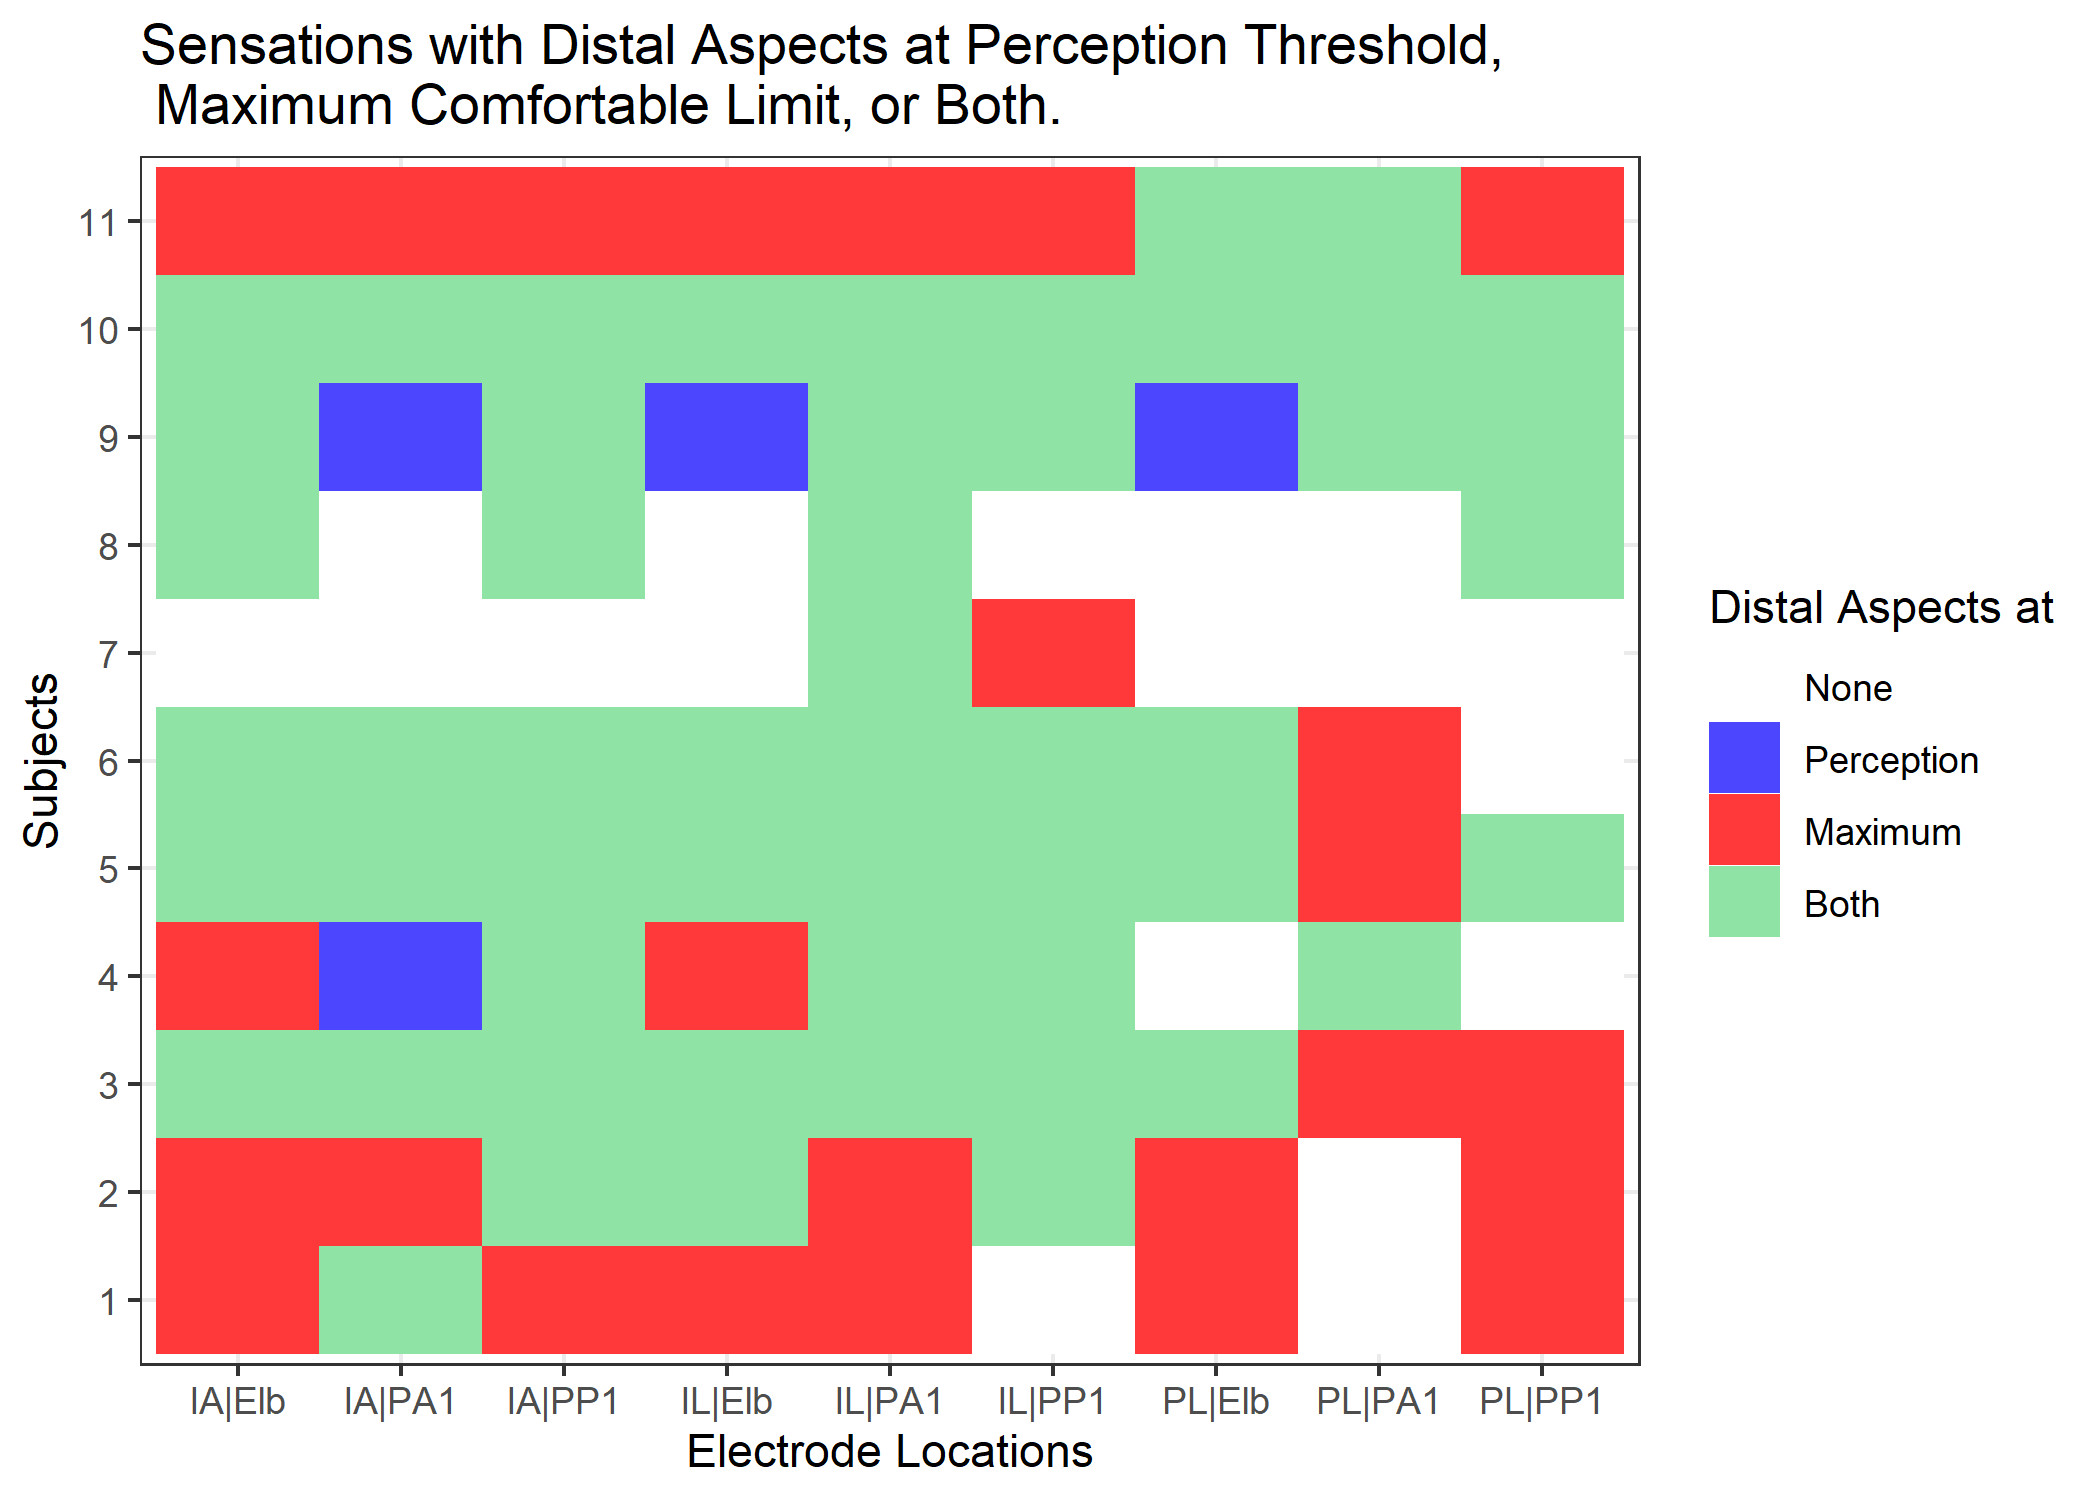
\includegraphics[width=0.5\textwidth, trim={0cm 0cm 0cm 0cm} ,clip]{fig/distal_sens_subj.jpg}
  \caption{The graph shows which electrode combinations were able to generate distal percepts for each of the eleven participants and nine electrode combinations. The graph classifies each condition by whether a distal percept was generated at the perception threshold, maximum comfortable limit, both, or no distal percept was reported.}
  \label{fig:distal_eva}
\end{figure}

\section{Discussion}

This study evaluated surface electrical stimulation's ability to generate distally referred sensations in intact subjects, with the goal of eliciting sensations at the fingertip. The experiment investigated the effects of electrode position, stimulation intensity, and stimulation polarity on perceived sensation location. 

The results showed that finger-palm electrode combinations were most likely to elicit distally-referred sensations. The position of the electrodes on the finger and palm in the circumferential or anteroposterior direction also impacted the perceived location of the distally-referred sensations, but there were no consistent trends across subjects. We found that the stimulation intensity also had statistically significant effects on sensation location: increases in stimulation intensity led to increases in the sensation area, proximal shifts of the percept centroid, and movement of the distal boundary of the percept to more distal locations. We discovered that 71\% of perceived sensations were not polarity dependent, and that a larger return electrode positioned on the elbow eliminated sensation located near the return electrode and reduced proximal sensations located on the palm. 

\subsection{Effects of Electrode Positions on Perceived Sensation Location}

The finger-palm combinations elicited distally-referred percepts isolated to the index finger. This distinguishes the current approach from previous sensory restoration studies, which placed electrode combinations on or proximal to the wrist and elicited sensations on large sections of the hand spanning multiple fingers \cite{slopsema_natural_2018, pena_channel-hopping_2021}. The current approach also elicited fewer instances of sensations in non targeted fingers or in the vicinity of the return electrodes (37\%, n=198), compared to prior studies that placed electrodes on the palm only ($\sim$55\%)\cite{dalonzo_electro-cutaneous_2018}. While there was some variability in reported sensory locations across participants for individual electrode configurations, we did find certain electrode configurations that consistently elicited distally-referred, comfortable sensation across participants.

The results from Experiment One suggested that the finger-palm electrode combination elicited distally-referred sensations more often than palm-palm or finger-finger combinations. A possible explanation for this difference is that the electric field was forced to travel more deeply in to the body to find a lower resistance path when the active and return electrodes were positioned farther away from each other (finger-palm). This result agrees with the literature, which has reported that deeper stimulation occurred as inter-electrode distance was increased \cite{gomez-tames_simulation_2012, kajimoto_electro-tactile_2016}. This would suggest that electrodes that are farther apart would be more likely to activate the digital nerve instead of the nerve endings close to the surface of the skin. Activating the digital nerves could generate a distally-referred sensation, but activating the local skin receptors may only generate a local sensation. These results suggest that the specific electrode combination is as important as the anatomical position of each individual electrode when eliciting sensory percepts.

The palm-palm location combination resulted in the lowest average percentage of instances of distally referred sensation, despite this electrode combination having inter-electrode distances comparable to those of the finger-palm combinations. When comparing across different palm electrode positions, electrodes positioned on more proximal areas of the palm were associated with a lower average percentage of useful sensations than electrodes on more distal areas of the palm. A possible explanation for this difference is that electrodes placed on more proximal areas of the palm were positioned over regions of the median nerve that innervate and elicit sensations on off-target non-index regions of the hand, which we instructed participants to classify as not useful sensations \cite{dalonzo_electro-cutaneous_2018, scarpelli_evoking_2020, tanaka_full-hand_2023}. This theory is supported by the observation that combinations including an electrode on the finger and an electrode at PA1 elicited useful sensations. PA1 is positioned on the distal area of the palm, so it is possible that electrode combinations involving this position are still able to selectively stimulate only the part of the median nerve that innervates the index finger. \citeauthor{dalonzo_electro-cutaneous_2018} also reported more sensations in off-target fingers during stimulation of proximal palm electrodes compared to electrodes in more distal areas of the palm \cite{dalonzo_electro-cutaneous_2018}. \cite{tanaka_full-hand_2023} also reported more distally-referred sensations limited to the target finger using a finger palm combination \cite{tanaka_full-hand_2023}. However, the anatomical position of their best individual electrodes were different. Experiment One included the electrode positions used by \citeauthor{tanaka_full-hand_2023}, but these positions did not perform as well in Experiment One as the positions we selected for Experiment Two. The difference in performance could be related to differences in stimulation intensities used during the exploratory studies (perception threshold vs. maximum comfortable limit) or the micro adjustments to the active electrode position performed by \citeauthor{tanaka_full-hand_2023} \cite{tanaka_full-hand_2023}. 

The exact location of the percepts varied greatly from participant to participant and across the electrode combinations, as shown by the standard deviation of the vertical centroid (Fig. \ref{fig:all_cent}). Also, no single electrode combination worked across all participants (Fig. \ref{fig:distal_eva}). Instead, each participant had a variation of the finger-palm pattern that worked best for them. Therefore, if this technology would to be implemented as a haptic device for MR applications, the wearable component of the device that positions the electrodes would have to have multiple electrode combinations available, adjustable electrodes, or current steering mechanisms in order to ensure finger percept locations for each user \cite{tanaka_full-hand_2023}.

\subsection{Effects of Stimulation Intensity on Perceived Sensation Location}

As stimulation intensity increased, the percepts had variable responses, so there was no consistent pattern across subjects. On average across subjects, when intensity increased, the percepts expanded across the index finger area, and stimulation at the maximum comfortable limits generated sensations with more distal aspects compared to stimulation at the perception thresholds. This increase in percept envelope size when increasing stimulation intensity is consistent with the literature \cite{dalonzo_electro-cutaneous_2018, graczyk_neural_2016, slopsema_natural_2018, scarpelli_evoking_2020}.

Also, the difference in pulse width and pulse amplitude across subjects could have influenced sensation location for electrode combinations with a greater inter-electrode distance, because as  the current required to initiate action potentials increases with inter-electrode distance \cite{doheny_effect_2010}. Experiment One was performed at the maximum comfortable limit of each subject for each electrode combination. Increasing inter-electrode distance could allow the participant to tolerate higher stimulation intensities and increase the stimulation depth, leading to  higher incidences of distally referred sensations.

All nine electrode combinations evaluated in Experiment Two elicited percepts mainly focused on the index finger on all subjects at both the perception threshold and the maximum comfortable limit. This is important because it shows that sensation intensity can be modulated over a wide dynamic range during MR/VR task performance while retaining distally-referred, selective, fused sensations.

\subsection{Sensation Intensity and Perceived Sensation Location}

All nine electrode combinations tested in Experiment Two were able to elicit distally-referred sensation on the index finger. While sensation intensity often varied across the percept, such that some regions of the percept felt stronger than others, typically the most intense sensations reported in each trial included the distally-referred aspects of the reported percepts. This was true for both threshold and maximum comfortable percepts, and suggests that the distally-referred aspects were the most noticeable or salient portions of the sensations and thus could be useful despite concurrent proximal or off-target sensation. 

\subsection{Effects of Electrode Polarity on Perceived Sensation Location}

Another key observation was that polarity had minimal effect ($<30\%$) on the sensory locations for the same electrode configuration. On symmetric waveforms, stimulation flipping the positions of the electrodes has the same effect as polarity inversion (cathodic vs. anodic), and the electrode with anodic stimulation will have higher thresholds \cite{koivuniemi_asymmetric_2011}. These higher thresholds explain the instances of polarity dependency. However, these trials were performed at the maximum comfortable limit, so even with higher thresholds, there is a possibility that the maximum comfortable limit was able to generate action potentials at both electrode sites. The sensation details (size, intensity, quality) are likely polarity dependent, but the presence of any type of sensation around the electrodes and therefor its classification as useful might not be polarity dependent. \citeauthor{kajimoto_electro-tactile_2016} also reported that anodic stimulation has higher thresholds for nerves running parallel to the skin, but lower thresholds for nerves running perpendicular to the skin (nerve terminals of Meissner’s corpuscles) than cathodic stimulation. These findings reinforce the theory that sensations can be present on both electrodes regardless of polarity at high stimulation intensities. 

The polarity independence caused by the high intensity symmetric waveform might have affected the results by excluding possible useful electrode combinations by eliciting sensations outside the index finger (palm). We implemented the elbow electrode as a possible mitigation strategy, but another possible mitigation strategy could be asymmetric waveforms which are more susceptible to polarity inversion than to flipping the electrode positions \cite{koivuniemi_asymmetric_2011}.

\subsection{Effects of an Asymmetrically Sized Elbow Electrode on Perceived Sensation Location}

A larger elbow return electrode eliminated percepts in the vicinity of the return electrode and reduced sensations located outside the targeted finger. Furthermore, none of the participants reported sensation at the return electrode when it was placed at the elbow. This could have been caused by the increased inter-electrode distance, increased electrode size, the change in electrode position, or a combination of these changes. Increasing the distance between the active and return electrodes and using a larger return electrode compared to the active electrode changes the stimulation from bipolar to monopolar \cite{plonsey_bioelectricity_2007,north_glossary_2022}. Other studies have reported higher threshold currents for larger electrodes, so size could decrease the likelihood of sensation on the return electrode \cite{cao_3-d_2014, gomez-tames_simulation_2012}. The return electrode was placed at the medial epicondyle of the elbow, a position far away from major nerves. The increased distance between the electrode and the nerves could increase the stimulation threshold.

The elbow electrode did not have any statistically significant effects on distally-referred sensations when compared to the other two return electrodes evaluated in Experiment Two. The literature suggested that increasing inter-electrode distance increased stimulation depth and the likelihood of stimulating the digital nerve \cite{gomez-tames_simulation_2012, kajimoto_electro-tactile_2016, tanaka_full-hand_2023}. This hypothesis would suggest that the electrode combinations with a return at the elbow return electrode would be more likely to elicit sensations with distally-referred aspects. However, the results from Experiment Two did not show a significant difference among the different return electrode positions. The lack of a difference might be due to the nerves in the finger being close to the surface of the skin, so deeper stimulation and inter-electrode distance would have a limited effect. Since all the evaluated electrode combinations reported distally-referred aspects, the digital nerve could have already been stimulated by combinations with return electrodes on the palm. 

\subsection{Limitations and Future Work}

A limitation of this study was that only the index finger was evaluated, so we did not evaluate whether our findings are consistent for other fingers. However, the limited exploratory tests performed for and during the semifinal entry to the Avatar XPRIZE competition showed that the electrode combinations explored during this paper using the elbow return electrode were applicable to the other fingers, with similar results \cite{zhangoperator}. Also, both experiments were limited by the use of a stimulator that outputs only symmetric waveforms. As explained before, a symmetric waveform may have caused some electrode combinations to produce sensation at both the active and return electrodes. Furthermore, the results of polarity dependence are limited by the simplification of the sensation to useful or not. This limitation could be addressed in future work by using a different stimulator that could be programmed to output asymmetric charge-balanced waveforms. A limitation of Experiment Two was that the three changes (size, location, inter-electrode distance) made to the elbow return electrode were evaluated simultaneously, so the results cannot be used to determine which changes successfully mitigated sensations around the return electrode.  

This study was an initial evaluation of how electrode position combinations distal to the wrist and stimulation parameters interacted to impact perceived location and intensity of evoked sensory percepts. In the future, these results could be used to develop a device to deliver haptic feedback for various applications in MR and VR, such as gaming, robotic surgery, and job training. While this study evaluated how percepts varied across participants, it would also be important to evaluate how percepts change over time within participants to optimize the calibration procedure for a future DR-SENS haptic device. In future work, we also plan to evaluate sensations evoked by DR-SENS in other fingers beyond the index, and determine whether the findings regarding electrode position hold across fingers.  

\section{Conclusions}

This study introduced a novel DR-SENS approach and evaluated the effects of electrode placement, polarity, and stimulation intensity on its ability to elicit distally-referred sensations in able-bodied individuals.  

We determined that electrode positions distal to the wrist can consistently evoke distally referred sensations with no significant polarity dependency. Within these different electrodes positioned distally from the wrist, the finger-palm combination performed the best, and the different variations of this combination did not have a significant effect. Increasing stimulation intensity significantly expanded the area of the sensation, moved the most distal sensation distally, and moved the vertical centroid proximally. Furthermore, this study showed that the most intense sensation for a given percept can be distally referred. Lastly, for each subject, at least one of the finger-palm combinations evaluated in this study worked at both stimulation intensities. 

These findings are a first step in understanding how to best apply DR-SENS for use as a tactile haptic display modality. The new knowledge generated by this study, along with the new questions that were identified, support further investigations of DR-SENS.

\section{Acknowledgements}

We thank the Cleveland FES Center for providing illustrations. This work was partially supported by National Science Foundation Grant 1942402. All the authors are listed as inventors on a pending patent of the technology described in this paper. Dr. Dustin Tyler owns equity in Afference Inc. which licensed the technology described in this manuscript. The data that supports the findings of this study are available upon reasonable request from the authors.


{\footnotesize
\bibliographystyle{myIEEEtranN}
\bibliography{zotero, manual_entries}}

\end{document}

